% AUTOGENERATED DRAFT from manuscript source: manuscript/chapters/08-diagnostics-cases.md
% Converter: scripts/convert_markdown_chapter_to_tex.py
% Review gate: docs/latex-migration-plan.md (Phase 2 per-chapter gate)

\chapter{诊断、验证与案例}
\label{chap:08-diagnostics-cases}

PIC 程序的可信度来自验证，而不是来自输入文件能跑完。一个最小验证闭环需要回答：

\begin{itemize}
\item 初始条件是否表达了目标物理问题；
\item 网格、粒子数、时间步是否分辨关键尺度；
\item 输出量是否足以检查守恒律和不稳定性；
\item 结果是否能和解析解、benchmark、regression 或文献对比；
\item 源码和分析脚本是否确实覆盖了所声称的运行路径。
\end{itemize}

本章不按文件格式罗列功能，而按一条读者可追踪的证据链展开：\textbf{先定义想测的物理量，再确认它从哪些运行态生成，接着选择 reader-side 的比较对象，最后标出该比较能支持和不能支持的结论。}Langmuir wave、uniform plasma 和 LWFA/PWFA 分别提供解析波、热背景与应用工作流三条主线；后半章再把同一方法落实到 full/reduced diagnostics、plotfile/openPMD/checkpoint 和边界粒子缓冲区。

\subsection{阅读路线：从物理问题走到证据等级}

本章的案例、writer 和 analysis 很多；第一次阅读不应按目录逐个收集输出类型，而应按以下顺序完成一个可解释的验证闭环：

\begin{enumerate}
\item \textbf{先读开头、Langmuir wave 与 Uniform plasma。} 从解析波、守恒量、热涨落或 restart 一致性中选定一个要测的 observable 和 reference；这一步回答“输出究竟要证明什么”。
\item \textbf{再按物理问题选案例族。} LWFA/PWFA、laser-target、capacitive discharge、reconnection 与束流应用分别给出不同的 producer 和模型边界。选择一个案例时，先写出它的初态、目标物理量和不可外推范围。
\item \textbf{随后读“诊断在源码中的位置”到案例模板。} 追踪 full/reduced diagnostics、plotfile/openPMD/checkpoint 和 boundary buffer 如何从运行态生成输出；这一步回答“这个量何时由哪个 consumer 写出”。
\item \textbf{最后读 8.14--8.17。} 把 physics gate、writer/schema contract、checksum 和 performance gate 分开，并用练习回查 producer、consumer、observable 与限制；这一步回答“通过或失败能支持什么结论”。
\end{enumerate}

因此，诊断设计的终点不是拥有更多文件，而是每个输出都有明确的问题、时间层、比较对象和证据等级。

\textbf{从第 7 章边界状态到第 8 章证据的交接卡。} 同一 time step 的输出并不天然代表同一采样时刻或同一组运行态。必须区分 back-transformed snapshot、普通 full/reduced diagnostics 与 boundary scraping 的 producer；否则会把 moving window 前的场、边界处理后的粒子和已清空的 scraping buffer 错接成一份“完整末态”。

\begin{enumerate}
\item \textbf{每步先建立 diagnostics 的迭代上下文。} \cpath{WarpX::Evolve()} 开始处调用 \cpath{multi\_diags->NewIteration()}，随后执行 \cpath{OneStep()} 的粒子/field 推进。back-transformed diagnostics 是例外：主循环先以 \code{multi_diags->FilterComputePackFlush(step, false, true)} 只分派 back-transformed 类型，再执行 \cpath{MoveWindow()} 与 \cpath{HandleParticlesAtBoundaries()}。因此 BTD 的 snapshot 不能自动被解释成完成 moving-window 位移或 particle boundary 后的普通末态。
\item \textbf{边界状态先形成，普通诊断随后读取。} \cpath{MoveWindow()} 后，\cpath{HandleParticlesAtBoundaries()} 才执行粒子 \cpath{ApplyBoundaryConditions()}、domain/embedded-boundary buffer 收集与重分配。electrostatic 或 Hybrid PIC 路径还会在这里之后计算步末 space-charge/Hybrid field；普通电磁路径的场已由前面的 \cpath{OneStep()} 完成。于是正常 full/reduced diagnostics 读取的是各自 solver 路径已经提交、并经过这段边界处理后的状态，而不是一次 field push 刚返回时的中间数组。
\item \textbf{速度时间层也要按诊断需求临时对齐。} 只要 \cpath{multi\_diags->DoComputeAndPack(step)} 或 \cpath{reduced\_diags->DoDiags(step)} 需要输出，且设置 \cpath{synchronize\_velocity\_for\_diagnostics}，主循环会调用 \cpath{SynchronizeVelocityWithPosition()}；下一步开始的半步 velocity push 会撤销这次对齐。因此同步后的粒子动量可以服务这一次指定诊断，不应被误当作永久改变的推进时间层。
\item \textbf{三类写出者的职责不同。} \cpath{reduced\_diags->ComputeDiags(step)} / \cpath{WriteToFile(step)} 先形成归约量；随后普通 \cpath{multi\_diags->FilterComputePackFlush(step)} 对 full diagnostics 判断是否 \cpath{ComputeAndPack()} 和 \cpath{Flush()}。\cpath{BoundaryScrapingDiagnostics::DoComputeAndPack()} 则固定返回 false：它只在 dump interval 把第 7 章已经收集的 boundary buffer 写入按边界命名的目录，然后清空 buffer。一个普通 plotfile、一个 reduced energy 文件和一份 scraped-particle 输出因而不是可互换的同一证据。
\end{enumerate}

验证时先将 observable 对齐到 producer：PML/PEC 场量使用时间层一致的 full 或 reduced field consumer，restart 比较恢复后的同类型输出，边界粒子问题必须读取 scraping 输出本身，BTD 还要明确其 snapshot/moving-window 约定。任何一份末态 plotfile、reduced scalar 或空的 scraping 目录都不能单独证明边界、场和粒子三条路径同时正确。

在进入具体案例前，可以先记住 Dawson 1983 对 diagnostics 的一个老判断：simulation 的目标是 physics essence，而不是 detail。也就是说，diagnostics 的价值不在于“把所有字段和粒子都写出来”，而在于能否把大规模数值状态压成可解释的 observables、谱、守恒量和 reader-side 证据。对二维和三维模型，这种 diagnostics / visualization / postprocessing 的难度甚至可能不低于模型本身。WarpX 的 full diagnostics、reduced diagnostics、back-transformed diagnostics、checkpoint 以及 openPMD/plotfile reader-side analysis，都不该只按 writer 类型分类，而应按“是否真正提炼出目标 physics”来理解。

同一篇综述还给了 diagnostics 的另一条很有价值的组织方式：先分 \code{measurements related to particle motion}，再分 \code{measurements related to waves}。前者典型的是 distribution function、phase space、drag、velocity diffusion；后者典型的是 field fluctuation level、time correlations、power spectrum 与 nonuniform-plasma normal modes。这种分法比“plotfile/reduced/openPMD/BTD”更接近物理问题本身，因为它直接对应读者真正要问的量：是想测输运系数、相关时间、噪声底、谱线，还是想重建某个本征模的空间结构。后面各案例如果只停在“输出了哪类文件”，而不说明它到底在测哪一类物理量，diagnostics 章节就会失焦。

\code{Dawson 1983} 后面的统计理论 examples 又把这条 diagnostics 思路压得更具体：这些 drag、diffusion、field-fluctuation 和 correlation measurements，不只是“可以输出的量”，而是 simulation 用来直接检验 subtle plasma statistics 的观测合同。作者甚至特意把一维 electrostatic sheet model 提出来当高精度 benchmark，因为它不需要 grid、可把 point-particle dynamics 跟到近 machine accuracy。于是 diagnostics 章节里有一条很值得保留的边界：reader-side analysis 的对照对象不一定只有解析式，也可以是更 fundamental、近 exact 的 particle model。这一点对后面理解 noisy thermal backgrounds、transport coefficients 和 fluctuation measurements 特别重要。

把这条统计 diagnostics 再压实一点，Dawson 给出的最小测量合同其实已经很完整：

\begin{itemize}
\item drag
\begin{itemize}
\item 不是看单粒子轨道，而是固定窄速度窗口后测群体平均速度衰减；
\end{itemize}
\item velocity diffusion
\begin{itemize}
\item 不是任意时段都能读系数，而要先识别 $\tau^2$ 的 short-time regime 和 decorrelation 后的近线性 regime；
\end{itemize}
\item field fluctuations
\begin{itemize}
\item 不是先看整张场图，而是先看每个 \cpath{k} mode 的 time-averaged modal energy 是否满足热平衡与 shape-modified fluctuation 预期。
\end{itemize}
\end{itemize}

这条合同对本书案例的意义很直接：后面不论是 \cpath{uniform\_plasma} 的 noisy thermal background、Langmuir family 的 fluctuation floor，还是 thermal-plasma energy/stability families，都更应该被组织成“这些 reader-side measurements 能否稳定恢复理论里真正关心的统计量”，而不是“导出了哪些字段文件”。

如果再往前推进一层，Dawson 的 wave-side diagnostics 还要求继续区分：

\begin{itemize}
\item power spectrum：
\begin{itemize}
\item 是 Debye-cloud random continuum 还是 collective plasma spike；
\end{itemize}
\item time correlations：
\begin{itemize}
\item 对应的 wave memory / decorrelation time 多长；
\end{itemize}
\item magnetized peaks：
\begin{itemize}
\item 是 Bernstein、upper-hybrid、ion-cyclotron、lower-hybrid，还是 $\omega=0$ 的 convective-cell / charged-flux-tube 结构。
\end{itemize}
\end{itemize}

这对本章的直接约束是：thermal / noisy plasma diagnostics 不该只停在 field RMS 或总场能量上，而应继续追问谱线形状、linewidth、相关时间和 peak taxonomy。否则我们只能知道“有噪声”，却不知道噪声究竟来自随机 continuum、热平衡模、磁化谐波，还是低频结构化 cells。

对 nonuniform plasma，Dawson 又把这条 diagnostics 合同推进了一步：reader-side analysis 的目标不只是标出某个 $\omega$ 上“有一条峰”，而是重建该峰对应的空间波函数。做法是先记录 $\phi(\mathbf r,t)$、$\mathbf E(\mathbf r,t)$ 或 $\mathbf B(\mathbf r,t)$；若系统在某个方向上均匀，就先沿该方向 Fourier 分解，再在剩余坐标上分析 $\phi(k_x,y,\omega)$ 这类量。对离散谱线 $\omega_1$，可以把信号分别与 $\sin\omega_1 t$ 和 $\cos\omega_1 t$ 做相关积分，从而恢复 mode amplitude 和 phase profile。这里有个很硬的 measurement boundary：积分窗口 $T$ 必须短于该 mode 的 damping time，否则初始 coherent oscillation 衰减后、由随机粒子运动重新激发的任意相位会把空间相位结构洗掉；长运行应拆成多个短窗口再平均，而不是简单延长一次积分。对连续谱也不能一概当噪声处理，因为其中既可能出现局域在某一小块等离子体区域的 localized oscillations，也可能只是 random particle motion 的 continuum；后者就必须继续测 $\delta v(\mathbf v,x,\omega)$ 这类 kinetic quantity，而不能只停在势场或电场谱图。

这一点又和 noisy start / quiet start 的工程边界连在一起。Dawson 明确指出，对 weak instability，random start 的主要问题不只是“图更吵”，而是它会直接限制增长率测量的动态范围：给定 $k$ 模的初始涨落通常是 $N^{-1/2}$ 量级，而弱不稳定最终可能只长到不到百分之一到几个百分点，于是总共可用的指数增长窗口只有有限的 $\gamma t$。作者给出的数量级判断是 $\gamma t \sim \frac{1}{2}\ln N$；即便 $N=10^5$，典型也只有大约 \cpath{5} 个 e-foldings，因此增长率往往只能测到二十个百分点量级，对更弱的不稳定性甚至会被 natural noise 直接淹没。更具体地说，纯随机空间加载还会强烈过激发 small-$k$ long-wavelength electrostatic modes，因为它没有体现 Debye shielding 和局域电中性；这说明 quiet-start 或 cell-neutral loading 的意义不只是“让初值更平滑”，而是把 weak-effect measurements 的可识别动态范围从噪声底里救出来。

\subsection{Dawson 统计诊断链：从 modal energy 到 normal-mode reconstruction}

Dawson 1983 的统计理论 examples 还给出了一条可以直接移植到现代 reader-side analysis 的 wave-side 诊断链。第一层不是把整张场图压成一个 RMS，而是对每个 Fourier mode 计算 time-averaged modal energy；第二层把同一 mode 的时间序列变成 power spectrum，用来区分随机粒子运动形成的连续谱和 collective plasma oscillation 形成的离散尖峰；第三层计算时间相关函数，测量 phase memory 和 decorrelation；第四层在非均匀等离子体中重建 mode 的空间波函数。四层分别回答“能量有多大、是哪类频率结构、记忆持续多久、空间上究竟是哪一个本征模”。

对单个波数 \cpath{k}，相关函数可写为

\[
C(k,\tau)=\lim_{T\to\infty}\frac{1}{T}\int_0^T E(k,t)E(k,t+\tau)\,dt,
\]

其对应的谱密度满足 Wiener--Khintchine 型关系

\[
G(k,\omega)=4\int_0^\infty C(k,\tau)\cos(\omega\tau)\,d\tau.
\]

因此 power spectrum 和 time correlation 不是两个互不相关的后处理图，而是同一 fluctuation process 的频域/时域表示。有限 run length $T$ 还给出不可绕过的频率分辨率边界 $\Delta\omega\simeq 1/T$：如果 $1/T$ 大于目标谱线宽度，所谓 peak width 主要是窗函数和有限样本造成的，不能直接当成物理 damping rate。对长期运行，应按多个短窗口分别估计，再把统计量汇总，而不是盲目延长一个相位已经失真的积分窗口。

在磁化等离子体中，peak taxonomy 本身也是物理结果。Bernstein harmonics、upper-hybrid、ion-cyclotron、lower-hybrid，以及 $\omega=0$ 附近的 convective-cell / charged-flux-tube 结构，不能统一归类为“噪声峰”；它们需要结合外磁场、species mobility 和空间结构共同解释。对非均匀等离子体，若沿均匀方向先做 Fourier 分解，可在剩余坐标上构造 $\phi(k_x,y,\omega)$；再把离散频率 $\omega_1$ 的信号分别与 $\sin\omega_1t$、$\cos\omega_1t$ 做相关积分，就能恢复 mode amplitude、phase 和空间波函数。这里的积分窗口必须短于该 mode 的 damping time，否则初始 coherent oscillation 衰减后，随机粒子运动重新激发的任意相位会把空间结构洗掉。

continuous spectrum 也不能自动当成无意义的背景。它可能包含局域在某一小块等离子体区域的真实振荡，也可能只是随机粒子运动的 continuum；后者需要进一步观察 $\delta v(\mathbf v,x,\omega)$ 等 kinetic observable，而不是只凭势场或电场谱下结论。对 weak instability，随机初态的 $N^{-1/2}$ 模涨落还会消耗可用的指数增长窗口，数量级上 $\gamma t\sim\frac12\ln N$；quiet-start / cell-neutral loading 的价值因此是提高可识别动态范围，而不是保证所有后续演化都更物理。上述统计链来自 Dawson 1983 的相关章节；它支撑的是 diagnostics 设计原则，不替代 WarpX 各案例已有的具体 runtime gate。
此外，\code{Birdsall 1985} 的 \cpath{13-6} 提醒我们：即使线性介电关系显示稳定，相对漂移仍可能把自由能转入非线性相空间 clump 与 density hole；因此接近稳定阈值的案例还应保留 phase-space correlation 观察，而不能只看场能量或把它直接归类为 NCI。

再往实现层压一步，Dawson 给的 quiet-start recipe 也不是抽象建议，而是明确的 phase-space construction：把相空间切成 cells，把每个空间 cell 内的目标速度分布 \cpath{P(v)} 归一到该 cell 的粒子数，再把 \cpath{P(v)} 分成等面积小区间，每个区间放一个粒子并赋予相应代表速度。对任意目标分布，还可以先构造 cumulative map \codeesc{y(v)=\textbackslash\{\}int\_\{-\textbackslash\{\}infty\}\textasciicircum{}\{v\}P(v')\textbackslash\{\},dv'}，再用其反函数把 \code{[0,1]} 上的均匀变量映射成所需速度分布。这说明 diagnostics 一侧讨论 noisy/quiet starts 时，不能只写“quiet start 降噪”，还要看到它真正交换掉了什么：它用更规则的有限粒子 phase-space covering 换取更大的 weak-effect dynamic range，但简单的 equal-area placement 对 tail 或低密度关键区域的分辨能力有限，于是后面才需要 weighted particles / many-size electrons 继续补这条短板。

\section{Langmuir wave}

入口：\cpath{Examples/Tests/langmuir/inputs\_test\_1d\_langmuir\_multi}

关键设置：

\begin{itemize}
\item \code{max_step = 80}
\item \code{geometry.dims = 1}
\item \code{boundary.field_lo = periodic}
\item \code{boundary.field_hi = periodic}
\item \code{algo.field_gathering = energy-conserving}
\item \code{algo.current_deposition = esirkepov}
\item 电子和正电子两个 species，密度 \code{n0 = 2.e24}
\end{itemize}

这个例子适合检查等离子体振荡频率、沉积和 Gauss 定律误差。输入中定义

\[
\omega_p=\sqrt{\frac{2n_0 e^2}{\epsilon_0 m_e}},
\]

这里的因子 2 来自电子和正电子两种可动带电粒子的对称贡献。动量微扰用正负相反的三角函数给出，使两个 species 产生相反响应。

图 8-1 给出 81 个快照序列末态的数值电场与解析场对照。两幅图使用同一纵轴尺度：左图为 simulation，右图为 theory。这个图只承担 reader-side 的波形 sanity check；严格的场误差、最终 Gauss-law 误差和频率拟合数值仍以紧随其后的 gate 为准。

\begin{figure}[htbp]
\centering
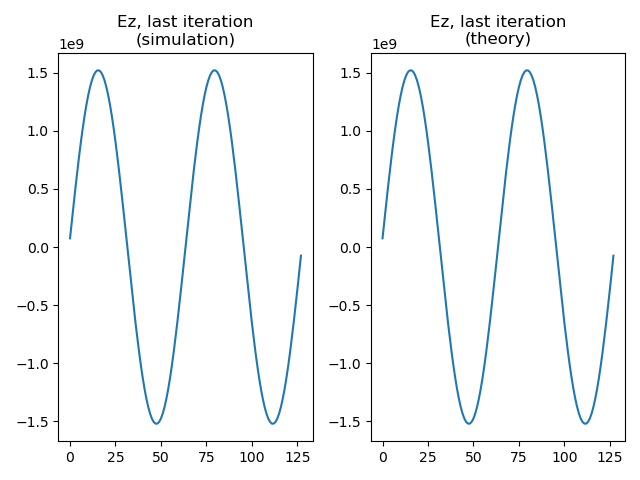
\includegraphics[width=0.8\linewidth]{../assets/figures/langmuir-field-vs-theory.png}
\end{figure}

图 8-1 由官方 Langmuir 输入和 reader-side analysis 生成；发布图像位于 \cpath{manuscript/assets/figures/}，正文不依赖临时运行目录。

Langmuir 验证树已经比这个 1D 入口更大。1D/2D/3D/RZ 原生输入族分别复用 \cpath{analysis\_1d.py}、\cpath{analysis\_2d.py}、\cpath{analysis\_3d.py}、\cpath{analysis\_rz.py}，因此共享同一个“解析场解逐点比较”的主合同；其中 3D 版本还额外检查 selective particle output 和 openPMD 粒子位置上的 \cpath{Ex/Ey/Ez} 场采样。\cpath{analysis\_utils.py} 又把 charge-conservation 检查做成条件分支，只在 Esirkepov、Vay deposition 或 PSATD current-correction 这些适用组合下强制比较 $\nabla\cdot\mathbf E$ 与 $\rho/\epsilon_0$。与之并列的 \cpath{langmuir\_fluids} 则是另一棵冷流体验证树：它不只看 \cpath{E}，还把 \cpath{J} 和 \cpath{rho} 一起与解析冷流体解比较。需要单独记住的是，2D/3D/RZ 的 PICMI 变体目前大多仍是 \cpath{analysis=OFF} 的前端 + checksum scaffold，不应和原生输入的强物理断言混成同一等级。

从应用综合章的角度，Langmuir wave 的价值不只是“有一个 textbook 解析解”，而是它把四条核心数值主线挂到了同一个最小物理问题上：

\begin{enumerate}
\item 初始化
\begin{itemize}
\item \cpath{NUniformPerCell}
\item \code{profile = constant}
\item \cpath{parse\_momentum\_function}
\end{itemize}
\end{enumerate}
共同决定冷等离子体微扰如何进入粒子。
\begin{enumerate}
\item 粒子推进与沉积
\begin{itemize}
\item \code{energy-conserving gather}
\item \cpath{Esirkepov}、\code{Vay deposition}
\item \code{momentum-conserving gather}
\end{itemize}
\end{enumerate}
在这个最小问题上暴露 $\nabla\cdot\mathbf E-\rho/\epsilon_0$ 误差。
\begin{enumerate}
\item 场求解
\begin{itemize}
\item FDTD
\item PSATD
\item \cpath{current\_correction}
\item \cpath{JRhom}
\end{itemize}
\end{enumerate}
都能在同一解析波形下做最小分支验证。
\begin{enumerate}
\item 诊断与 reader-side analysis
\begin{itemize}
\item plotfile/full diagnostics
\item openPMD
\item selective particle output
\item on-particle \cpath{Ex/Ey/Ez}
\end{itemize}
\end{enumerate}
都已经有现成 analysis 脚本消费。

这也是为什么 \cpath{Examples/Tests/langmuir/} 不只是一个普通回归目录，而是应用综合章最适合先理解的第一条主线。它把：

% <-- fenced code (text)
\begin{codeblock}
冷等离子体解析振荡
-> parser 初始化
-> gather / pusher / deposition / solver
-> diagnostics / openPMD reader
-> MR / PSATD / current correction / JRhom / PICMI / fluids 分支
\end{codeblock}

压在了同一个最小问题上。

归档的 1D 运行产物表明，这条主线不只停在源码和 analysis 脚本层；它产生 \cpath{diags/diag1000080}，并可用同一组解析式复核核心断言：

\begin{itemize}
\item 解析场相对误差 \code{error_rel = 1.70e-3 < 5e-2}
\item $\nabla\cdot\mathbf E-\rho/\epsilon_0$ 相对误差 \code{8.35e-12 < 1e-11}
\end{itemize}

因此 \code{Langmuir wave} 是运行级强基准，而不只是“源码上看起来应该能验证”的基准。读者可从 \cpath{Examples/Tests/langmuir/inputs\_test\_1d\_langmuir\_multi} 出发，用与所用 WarpX 版本匹配的 build 和 \cpath{analysis\_1d.py} 重建同一条验证链；后文的频率拟合说明补充了逐快照证据。

\section{Uniform plasma}

入口：\cpath{Examples/Physics\_applications/uniform\_plasma/inputs\_test\_2d\_uniform\_plasma}

关键设置：

\begin{itemize}
\item \code{max_step = 10}
\item \code{geometry.dims = 2}
\item 周期场边界
\item 单电子 species
\item 常密度 \cpath{1.e25}
\item gaussian 动量分布，\code{ux_th = uy_th = uz_th = 0.01}
\end{itemize}

这个例子更适合检查并行分解、粒子噪声、诊断输出和性能路径。因为物理结构简单，任何明显的非均匀场增长、粒子丢失或能量异常都容易被发现。

但 \cpath{uniform\_plasma} 目录里的 regression 边界需要写得更精确。\cpath{test\_2d\_uniform\_plasma} 和 \cpath{test\_3d\_uniform\_plasma} 在 \cpath{CMakeLists.txt} 中都没有独立 analysis，实际只依赖顶层 \cpath{Examples/analysis\_default\_regression.py} 提供 checksum 基线；因此它们更像是“full diagnostics / 并行噪声 / 最小工作流稳定性”基准，而不是独立的热等离子体物理 hard assert。真正的强断言在 \cpath{test\_3d\_uniform\_plasma\_restart}：它从 \cpath{chk000006} 恢复，再用 \cpath{Examples/analysis\_default\_restart.py} 逐字段比较 restart 与非 restart 输出，要求相对误差低于 \cpath{1e-12}。另外，名字里带 \cpath{uniform\_plasma} 的 \cpath{test\_3d\_uniform\_plasma\_psatd\_JRhom\_CC1} 并不属于这个应用目录，而是 \cpath{nci\_psatd\_stability} 里的 PSATD 稳定性回归，它检查的是 \code{JRhom=CC1 + div cleaning} 后电场能量是否足够小，从而证明 NCI 被压制，而不是均匀热等离子体本身的统计性质。

这意味着 \cpath{uniform\_plasma} 在应用综合章里最准确的角色不是“单一 physics benchmark”，而是最小热背景 workflow：

\begin{enumerate}
\item 均匀、周期、单 species 的 thermal background
\begin{itemize}
\item 给粒子噪声和并行划分提供最低复杂度基线；
\end{itemize}
\item full diagnostics
\begin{itemize}
\item 给 plotfile/openPMD 风格输出提供最小 reader-side 骨架；
\end{itemize}
\item checkpoint/restart
\begin{itemize}
\item 给 \cpath{analysis\_default\_restart.py} 提供一条极干净的 field-level reproducibility 基准。
\end{itemize}
\end{enumerate}

若把“噪声、能量、性能和诊断”拆开，证据来源其实是分层的：

\begin{itemize}
\item 噪声、性能背景、writer/checkpoint：
\begin{itemize}
\item 主要来自 \cpath{Examples/Physics\_applications/uniform\_plasma/}
\end{itemize}
\item 热等离子体总能量强断言：
\begin{itemize}
\item 主要来自相邻 \cpath{Examples/Tests/energy\_conserving\_thermal\_plasma/}
\end{itemize}
\item PSATD/JRhom 稳定性强断言：
\begin{itemize}
\item 主要来自相邻 \cpath{Examples/Tests/nci\_psatd\_stability/}
\end{itemize}
\end{itemize}

因此 \cpath{uniform\_plasma} 的真正价值，不是它自己包含了所有强 analysis，而是它把：

% <-- fenced code (text)
\begin{codeblock}
均匀热背景
-> 粒子噪声 / 并行稳定性
-> full diagnostics / checkpoint
-> restart reproducibility
-> 与能量守恒、PSATD 稳定性测试树的边界
\end{codeblock}

压成了本书第二条适合系统学习的应用主线。

\cpath{test\_2d\_uniform\_plasma} 的 CTest 注册为 2-rank，但不带独立 analysis，只附加 \cpath{analysis\_default\_regression.py} 的 checksum。它因此是一个很有价值的最小 workflow 基线：可以检查输入、并行分解和 Full diagnostics 能否共同产出预期输出；却不能把 checksum 通过写成热等离子体能量守恒，也不能因为输入生成了 Full diagnostic 就宣称已经完成了 openPMD reader 验证。需要后者时，应选择实际把 openPMD 作为 consumer 的案例。

\subsection{Checkpoint/restart 的读者合同：续跑一致性与跨布局比较不是同一问题}

\cpath{test\_3d\_uniform\_plasma\_restart} 才把这个应用从“能生成输出”推进到一条明确的续跑比较。它依赖 \cpath{test\_3d\_uniform\_plasma}，两者都注册为 3D、2-rank CTest：基线输入在第 6 步写出 \cpath{chk000006}，restart 输入只在同一输入上增加 \code{amr.restart = "../test_3d_uniform_plasma/diags/chk000006"}。两条路径都推进到第 10 步，并把同一类 Full diagnostic 写到 \cpath{diags/diag1000010}。

consumer 的定义比“比较两个文件”更严格。\cpath{analysis\_default\_restart.py} 从 restart 测试目录名去掉 \cpath{\_restart} 来定位基线目录；随后在两个 level-0 covering grid 上遍历基线的完整 \cpath{field\_list}。因此它同时消费网格场、粒子属性和诊断实际写出的字段，而不是只比较 \cpath{E} 的一张切片。对每个字段，它计算

\[
\epsilon_f = \frac{\max |f_{\rm restart}-f_{\rm base}|}{\max |f_{\rm base}|},
\]

当基线分母为零时保留绝对最大差；默认要求每一个字段满足 \code{epsilon_f < 1e-12}。这给读者一条可执行的续跑合同：先固定 build、输入、checkpoint、输出时间和并行布局，再比较基线与 restart 的同一末态。

这里必须把三种问题分开：

\begin{enumerate}
\item \textbf{续跑一致性：} 同一 CTest 布局下，checkpoint 是否保留了使后续场和粒子输出可重合的状态。这正是上述 consumer 检查的对象。
\item \textbf{跨布局比较：} 1-rank 与 2-rank，或不同分块、GPU/MPI 组合是否给出相同的统计量或场，并不是这个 restart consumer 的输入。它需要事先指定独立 observable、随机采样策略和容差，不能从 \code{epsilon_f < 1e-12} 自动推出。
\item \textbf{输出回归：} CMake 还为 restart sibling 添加了 \code{analysis_default_regression.py --rtol 1e-12}。checksum 能发现指定输出相对基线是否改变，但它不是基线/restart 同字段比较的替代品；两类失败也必须分别诊断。
\end{enumerate}

因此，这条测试可以支持“指定 3D、2-rank、checkpoint-to-restart 路径的末态输出可按 \cpath{1e-12} 合同比较”，不能支持热平衡已经守恒、任意 MPI 布局物理等价，或 checkpoint 覆盖了没有写入 \cpath{field\_list} 的任意外部状态。\cpath{uniform\_plasma} 的物理闭环仍需由 \cpath{energy\_conserving\_thermal\_plasma} 和 \cpath{nci\_psatd\_stability} 中各自的 observable 提供。

\section{激光与束流驱动的尾场加速}

尾场加速不应按源码目录名被拆成彼此无关的两个例子。读者面对的是同一个问题：一个相对论驱动在欠密度等离子体中建立纵向尾场，见证粒子能否在合适相位停留足够长时间而获得能量。两条分支的差别在于驱动者：

\begin{enumerate}
\item \cpath{LWFA} 用激光脉冲的有质动力驱动尾场；
\item \cpath{PWFA} 用相对论束团的空间电荷和电流驱动尾场。
\end{enumerate}

无论选哪一条分支，先把诊断问题写成四项，而不是先浏览输入文件：

\begin{enumerate}
\item 纵向场的幅度、相位和相速度是否与所用近似一致；
\item 见证粒子是否处于加速且聚焦的相位区，其能谱、能散和横向尺寸如何演化；
\item 驱动、尾场和见证束之间的能量流向是否可从同一诊断时序中闭合；
\item moving window、boosted frame、网格细化和前端选择是否改变上述物理量的解释，而非只改变输出文件。
\end{enumerate}

\cpath{Examples/Physics\_applications/laser\_acceleration/} 和 \cpath{Examples/Physics\_applications/plasma\_acceleration/} 是回到实现的两个入口；它们能够帮助读者定位这些数值设置，却不是自动成立的统一物理基准。

\subsection{LWFA：先用尺度关系建立可检验的问题}

\code{Tajima-Dawson 1979} 给出了激光尾场的最小物理链：

% <-- fenced code (text)
\begin{codeblock}
laser pulse -> ponderomotive wake -> trapping -> acceleration
\end{codeblock}

在线性、欠密度的起点上，它给出

\[
v_p = v_g^{EM} = c\sqrt{1-\frac{\omega_p^2}{\omega^2}},
\]

\[
L_t = \frac{\lambda_w}{2} = \frac{\pi c}{\omega_p},
\]

\[
eE_L \cong mc\omega_p,
\qquad
\gamma_{\max} \simeq 2\frac{\omega^2}{\omega_p^2},
\qquad
l_a \cong 2\frac{\omega^2 c}{\omega_p^3}.
\]

这些关系把相速度、dephasing、加速长度和驱动频率放到同一张量纲图上。它们适合用来提出量级和趋势的预期，不能直接代替现代 moving window、boosted frame、mesh refinement、openPMD 或 PICMI 输入的验证。

这篇早期工作还给出一个最小 relativistic electromagnetic PIC demonstration：\code{1 1/2-D}、一个空间维度、三个速度/场分量、Gaussian finite-size particles 和固定离子背景。通过扫描 $\omega/\omega_p$，文中的数值结果支持三个有限结论：

\begin{enumerate}
\item wake longitudinal field 可达到
\end{enumerate}
\[
   E_L \sim 0.6\,\frac{mc\omega_p}{e},
\]
即冷等离子体 wave-breaking 级上限的大约 \codeesc{60\%}；
\begin{enumerate}
\item driver spectrum 会裂成多峰，作者明确解释为 successive / multiple forward Raman scattering，并把它和 photon deceleration、wake emission 联系起来；
\item simulation 中的最大电子能量随 $(\omega/\omega_p)^2$ 的变化基本贴合解析式，只是在高端开始受有限系统大小和周期边界污染。
\end{enumerate}

它因此是理解 \cpath{LWFA} 尺度和最小电磁 PIC 证据的文献入口，而不是当代实现的回归说明。文中关于 1979 年工程可行性、two-laser / beat-wave alternative 以及 pulsar atmosphere 的讨论都属于历史语境，不能外推为现代单脉冲 \cpath{LWFA} 的结论。

WarpX 的 \cpath{laser\_acceleration} 目录让读者把上述问题落到 1D/2D/3D/RZ、moving window、boosted frame、细化区域、PICMI 和 openPMD 上。目录中可直接追踪的三条局部比较分别是：

\begin{enumerate}
\item \cpath{analysis\_1d\_fluid\_boosted.py}
\begin{itemize}
\item 检查 boosted 1D 冷流体 \cpath{Ez/Jz/rho/Vz} 是否贴理论；
\end{itemize}
\item \cpath{analysis\_refined\_injection.py}
\begin{itemize}
\item 检查 refined injection 的总粒子数和 refinement-edge 前方 \cpath{rho} 均匀性；
\end{itemize}
\item \cpath{analysis\_openpmd\_rz.py}
\begin{itemize}
\item 检查 RZ openPMD diagnostics 的 mesh shape、species ordering 和 \cpath{rho\_<species>} 物理中心。
\end{itemize}
\end{enumerate}

这些检查分别约束冷流体场量、细化注入附近的粒子分布和 RZ openPMD 数据的结构；它们没有共同断言尾场幅度、束流增益或激光衍射。因此读者应把该目录当作实现与诊断的入口，并自行为所研究的物理量增加比较对象。

\subsection{PWFA：把束团和见证束的相位关系放在前面}

\cpath{plasma\_acceleration/README.rst} 指向的是 beam-driven wakefield acceleration：驱动者是相对论束团，不是 laser antenna。阅读这类输入时，首先确认驱动束、等离子体密度坡和见证束的初始相对位置；再检查 moving window、boosted frame 与数值 Cherenkov 修正是否和拟研究的相位演化相容。

该目录覆盖的实现选择包括：

\begin{itemize}
\item moving window
\item boosted frame
\item rigid bunch
\item density ramp / plasma channel
\item \code{particles.use_fdtd_nci_corr = 1}
\item mesh refinement
\item hybrid grid
\item PICMI front-end
\end{itemize}

其中多数注册案例使用默认输出回归：它能发现同一输入下输出是否发生变化，却不构成尾场幅度、dephasing 或 beam loading 的解析验证。\cpath{README.rst} 还明确保留一个前端边界：3D PICMI 输入尚未像 native boosted 输入那样使用 boosted frame。因此它可作为 non-boosted PICMI 的搭建起点，不能被当作 native boosted PWFA 的等价实现。

\subsection{本节的证据边界}

两个目录共同覆盖 moving window、boosted frame、诊断、网格细化以及 PICMI/native 前端；它们不共同提供一个尾场物理基准。更稳妥的读法是：

% <-- fenced code (text)
\begin{codeblock}
先用解析尺度或文献给出场、相位和能谱的预期
-> 用输入文件确认驱动和数值设置
-> 用诊断构造同一组可比较量
-> 再判断特定案例是否回答了该物理问题
\end{codeblock}

这样，源码案例承担“如何搭建和输出”的职责，解析关系和独立参考承担“是否正确”的职责，二者不会互相替代。

\section{Laser ion / plasma mirror / RPA/TNSA}

这一条应用主线必须写得比目录名更谨慎。案例库中真正可落到 application tree 的 laser-target 入口只有两个：

\begin{itemize}
\item \cpath{Examples/Physics\_applications/laser\_ion/}
\item \cpath{Examples/Physics\_applications/plasma\_mirror/}
\end{itemize}

而 \cpath{RPA/TNSA} 当前并没有独立应用目录或回归树，只是：

\begin{itemize}
\item \cpath{laser\_ion/README.rst} 背后的物理机制标签；
\item \cpath{Docs/source/glossary.rst} 里的术语定义。
\end{itemize}

\subsection{\texttt{laser\_ion}：先检验诊断一致性，再讨论离子能谱}

\cpath{laser\_ion} 的真实角色不是“已经证明某条 ion-acceleration scaling”，而是：

\begin{itemize}
\item Gaussian laser
\item planar solid-density target
\item full diagnostics
\item time-averaged diagnostics
\item reduced diagnostics
\item PICMI front-end
\end{itemize}

这条组合工作流的应用入口。

注册的 \cpath{analysis\_test\_laser\_ion.py} 检查的是：

\begin{itemize}
\item \cpath{diagInst} 最后 5 个瞬时 \cpath{Ez} snapshot 的时间平均
\item 与 \cpath{diagTimeAvg} 的原位 time-averaged \cpath{Ez} 是否逐点一致
\end{itemize}

因此它最直接的 regression 合同是：

\begin{itemize}
\item diagnostics time-average consistency
\end{itemize}

而不是：

\begin{itemize}
\item TNSA cutoff energy
\item RPA threshold
\item ion conversion efficiency
\end{itemize}

README 中的 \cpath{analysis\_histogram\_2D.py} 和 \cpath{plot\_2d.py} 用于读者后处理，不是同一条数值比较本体。

还要保留一个前端边界：\cpath{laser\_ion} 有 PICMI 版输入，但其 reduced diagnostics 能力和 native 版并不完全对齐，例如 PICMI 脚本里仍留有 \cpath{ParticleHistogram2D} 的 TODO。因此更准确的说法是：

\begin{itemize}
\item PICMI 已覆盖主工作流与 \cpath{analysis\_test\_laser\_ion.py} 合同；
\item 但前端能力还没有完全追平 native input。
\end{itemize}

\subsection{\texttt{plasma\_mirror}：表面等离子体的搭建入口}

\cpath{plasma\_mirror} 当前应用语义很明确：

\begin{itemize}
\item laser-solid interaction
\item surface plasma
\item planar overdense target
\end{itemize}

这一案例的可比较量仍需读者自行定义：

\begin{itemize}
\item 只有 \cpath{test\_2d\_plasma\_mirror}
\item \code{analysis = OFF}
\item checksum helper
\item 没有 PICMI
\item \cpath{README.rst} 的 Analyze/Visualize 仍是 \cpath{TODO}
\end{itemize}

默认输出回归只能提供稳定输出的线索。因此它更适合承担：

\begin{itemize}
\item laser-solid surface-plasma workflow baseline
\end{itemize}

而不是：

\begin{itemize}
\item reflectivity benchmark
\item high-harmonic benchmark
\end{itemize}

\subsection{\texttt{RPA/TNSA}：机制标签，不是独立应用目录}

这条边界如果不写清，很容易把文献中的机制标签误写成案例库已有的独立 examples。最强、也最保守的结论只能是：

\begin{enumerate}
\item \cpath{laser\_ion}
\begin{itemize}
\item 是激光打固体平面靶的应用骨架；
\end{itemize}
\item \cpath{RPA/TNSA}
\begin{itemize}
\item 是理解这类骨架时需要引入的机制标签；
\end{itemize}
\item 当前 \cpath{Examples/} 中
\begin{itemize}
\item 没有独立 \cpath{rpa\_*}
\item 也没有独立 \cpath{tnsa\_*}
\end{itemize}
\end{enumerate}
application tree。

因此，这条应用综合章更准确的组织方式是：

% <-- fenced code (text)
\begin{codeblock}
laser-target applications
-> laser_ion
-> plasma_mirror
-> RPA/TNSA as mechanism labels, not standalone application trees
\end{codeblock}

\section{Capacitive discharge}

这条应用线不应混成普通 \cpath{collision/*} 附属条目。它更准确的角色是：

\begin{itemize}
\item \code{PIC-MCC low-temperature plasma application tree}
\end{itemize}

因为它同时把以下对象接到同一应用骨架上：

\begin{itemize}
\item parallel-plate electrostatic discharge
\item \cpath{background\_mcc}
\item 可选 DSMC ionization 分支
\item PICMI front-end
\item Python callback Poisson solver
\item Turner benchmark profile 对照
\end{itemize}

\subsection{1D PICMI：Turner profile 的直接比较入口}

两条注册案例是：

\begin{itemize}
\item \cpath{test\_1d\_background\_mcc\_picmi}
\item \cpath{test\_1d\_dsmc\_picmi}
\end{itemize}

它们共用同一条脚本：

\begin{itemize}
\item \cpath{inputs\_base\_1d\_picmi.py}
\end{itemize}

这不是普通薄输入卡，而是完整的 benchmark driver：

\begin{enumerate}
\item 选择 Turner case \cpath{N=1..4}
\item 组装 1D electrostatic grid
\item 可选安装 Python level Poisson solver callback
\item 打开 \cpath{background\_mcc}
\item 可选把 ionization 切成 DSMC
\item 累积离子密度并写出 \cpath{ion\_density\_case\_N.npy}
\end{enumerate}

\code{--test --pythonsolver} 是脚本支持的单独模式；它会显式确认：

\begin{itemize}
\item callback solver 已经实际运行；
\item \cpath{he\_ions} 的 \cpath{z} 坐标访问链可用。
\end{itemize}

但当前注册的两个 1D CMake 测试分别传入 \cpath{--test} 与 \code{--test --dsmc}，都\textbf{没有}传入 \cpath{--pythonsolver}。因此 active regression 能证明的是 MCC 或 DSMC 的离子密度验证和粒子坐标访问链；Python Poisson callback 是可单独运行的接口路径，不能被写成已经由这两条活跃测试覆盖。

因此这条应用树在工程上除低温等离子体 benchmark 外，还提供清晰的：

\begin{itemize}
\item PICMI + Python callback Poisson solver
\end{itemize}

可选应用入口；两种角色需要分别验证。

\subsection{可直接比较的量：case-1 ion-density profile}

两条当前注册的 1D 测试都调用 \cpath{analysis\_1d.py}。它直接读取：

\begin{itemize}
\item \cpath{ion\_density\_case\_1.npy}
\end{itemize}

分析器将脚本内 129 个节点的 Turner case-1 reference 插值到模拟网格，跳过两端吸收壁节点后计算 interior relative-error 的 RMS，并要求小于 \codeesc{6\%}。跳过边界不是放松物理比较：源码注释指出 nodal charge deposition 在吸收壁只看到半个 cell，端点约半值是离散边界伪影，不能与 cell-averaged benchmark 直接并列。

因此该案例最强的 physics contract 是：

\begin{itemize}
\item final averaged ion density profile
\item against Turner benchmark case 1
\end{itemize}

而不是笼统的“有 MCC test”或“有 DSMC test”。

\subsection{DSMC 版不是孤立小 test，而是同一 benchmark scaffold 的分支}

这两条 1D tests 共享同一应用骨架，区别只在于 collision realization：

\begin{enumerate}
\item \cpath{test\_1d\_background\_mcc\_picmi}
\begin{itemize}
\item \cpath{background\_mcc}
\item 默认 WarpX electrostatic solver，不是 CMake 传入的 Python callback
\item Turner case-1 profile 对照
\end{itemize}
\item \cpath{test\_1d\_dsmc\_picmi}
\begin{itemize}
\item 把 ionization 切到 DSMC 分支
\item 仍回到同一 Turner case-1 profile 对照
\end{itemize}
\end{enumerate}

因此更准确的表述是：

\begin{itemize}
\item DSMC 分支已经在同一低温等离子体 benchmark scaffold 里被强对照覆盖
\end{itemize}

而不是只证明“DSMC can run”。

\subsection{2D native / PICMI：搭建基线，不是 2D Turner 对照}

与 1D 的 profile 对照相比，2D 分支只有：

\begin{itemize}
\item \cpath{test\_2d\_background\_mcc}
\item \cpath{test\_2d\_background\_mcc\_picmi}
\end{itemize}

并且两者都是：

\begin{itemize}
\item \code{analysis = OFF}
\item checksum helper
\end{itemize}

因此它们只能作为：

\begin{itemize}
\item \code{2D capacitive-discharge workflow baseline}
\end{itemize}

而不是 2D Turner 强基准。另一个必须保留的边界是：

\begin{itemize}
\item \cpath{test\_2d\_background\_mcc\_dp\_psp}
\end{itemize}

整条 \cpath{add\_warpx\_test(...)} 仍被注释掉，所以它只能作为遗留分支记录，不能被当作已注册的比较案例。

\subsection{验证合同判读卡：相同的“通过”并不表示相同的正确性}

下面三条 active regression 都能给读者一个强比较量，但它们的 producer、reference 和结论范围完全不同。开始复现前，先选与你的问题同类的合同，而不是看到 \cpath{analysis.py} 就把它们视为等价验证。

% <-- table block (source: 08-diagnostics-cases L531)
\begin{tabularx}{\textwidth}{LLLLL}
\toprule
问题 & producer 与 consumer & 明确的通过条件 & 可以支持的结论 & 不能支持的结论 \\
\midrule
\endfirsthead
\toprule
问题 & producer 与 consumer & 明确的通过条件 & 可以支持的结论 & 不能支持的结论 \\
\midrule
\endhead
线探针是否保存了单缝衍射的横向包络 & \cpath{field\_probe} 的 \cpath{FP\_line} 是 201 点的 \cpath{FieldProbe} line detector；\code{integrate = 1} 使每步累加 $\lvert\mathbf S\rvert\Delta t$。\cpath{analysis.py} 在 step 500 从 \cpath{FP\_line.txt} 读取该积分量，以数值最大值归一后和单缝 $\mathrm{sinc}^2$ 包络比较 & 远离横向边缘的一组 probe 点的平均相对误差 \codeesc{< 2.5\%} & 在启用 EB 的该 2D 单缝设置中，line \cpath{FieldProbe} 的\textbf{归一化时间积分 Poynting-flux 形状}与解析包络一致 & 绝对光强标定、任意 probe geometry、boosted-frame lab-frame 数据，或 PML/粒子边界整体正确 \\
低温放电的平均离子密度是否接近外部 benchmark & 1D PICMI run 在最后诊断窗口逐步沉积并同步 \cpath{rho\_fp}，累积 \cpath{he\_ions} 密度后写出 \cpath{ion\_density\_case\_1.npy}；\cpath{analysis\_1d.py} 对插值后的 Turner profile 做 interior RMS 比较 & interior RMS relative error \codeesc{< 6\%} & 给定 case-1、1D electrostatic、MCC 或 DSMC 分支下，最终窗口平均 ion-density profile 与该 Turner 数据表相符 & Python Poisson callback 已由 active test 覆盖、任意 RF phase 的瞬时密度正确，或 2D discharge 已获得同一 benchmark 对照 \\
空间电荷限制二极管是否满足指定解析解 & 1D electrostatic Pierce diode 连续以 $J_{\rm CL}/q$ 注入离子，最终 \cpath{diag1} openPMD 写出 $\phi,E_z,\rho,j_z$；analysis 重建 Child--Langmuir 理论曲线 & $\phi$ 在首个非零节点之后、$j_z$ 在全比较网格上均满足相对误差 \codeesc{< 20\%} & 该平板、稳态、1D Child--Langmuir 配置的 potential 和 current-density 合同成立 & \cpath{E\_z}、\cpath{rho}、粒子相空间的同等强断言，任意发射模型，或 embedded-boundary ion extraction 已验证 \\
\bottomrule
\end{tabularx}

第一行的 \code{integrate = 1} 是一个容易误读的时间层细节：输出列的单位是 $\mathrm{W\,s/m^2}$，不是瞬时 $\mathrm{W/m^2}$。源码先在 probe 位置 gather $E/B$，计算 $\lvert\mathbf E\times\mathbf B\rvert/\mu_0$，再逐步乘 $\Delta t$ 累加；这个测试比较的是归一化空间\textbf{fluence} 包络。若研究的问题是某一时刻的场幅或频谱，应关闭积分或另设相应的时间序列 consumer，而不能沿用这条 \codeesc{sinc\textasciicircum{}2} gate。

第二、三行则展示了两种不同 reference。Turner profile 是离散表格，要求先处理网格插值和端点离散边界；Child--Langmuir 则是解析函数，$\phi(0)=0$ 会使相对误差没有定义，所以分析器从 \cpath{phi[1:]} 开始。二者都比 checksum 更接近物理比较，但它们只约束明确写入断言的 observable。读者复现实验时，应把输入模型、producer、consumer、reference、被排除的点和容差一起写入诊断记录卡；缺少其中任何一项，都不能把一次 PASS 推广成“该应用已经验证”。

\section{Magnetic reconnection}

磁重联这条应用线最准确的入口不是一般 \cpath{Fluids/}，而是：

\begin{itemize}
\item \cpath{Examples/Tests/ohm\_solver\_magnetic\_reconnection/}
\end{itemize}

它依赖的是：

\begin{itemize}
\item \cpath{picmi.HybridPICSolver}
\item \cpath{HybridPICModel}
\end{itemize}

也就是：

\begin{itemize}
\item kinetic ions
\item electron-fluid Ohm closure
\item Faraday + RK 子步推进 \cpath{B}
\end{itemize}

而不是 \cpath{WarpXFluidContainer} 那条额外 cold-fluid species runtime layer。这个边界必须写死，因为两条实现承担的职责不同：

\begin{itemize}
\item \cpath{Fluids/}
\begin{itemize}
\item 自己维护 nodal \cpath{N/NU}
\item gather 主场
\item 再把 \cpath{rho/J} 沉积回普通场寄存器；
\end{itemize}
\item \cpath{HybridPICModel}
\begin{itemize}
\item 则是在 field solver 内部从总电流、离子电流和电子闭合关系反推出 \cpath{E}。
\end{itemize}
\end{itemize}

因此 \cpath{magnetic\_reconnection} 在应用综合章里的正确角色是：

\begin{itemize}
\item \code{hybrid-PIC space-plasma application}
\end{itemize}

而不是：

\begin{itemize}
\item \code{fluid/PIC coupling demo}
\end{itemize}

\subsection{force-free sheet + reduced \texttt{FieldProbe}}

\cpath{inputs\_test\_2d\_ohm\_solver\_magnetic\_reconnection\_picmi.py} 不是薄输入卡，而是完整应用 driver。它同时定义了：

\begin{itemize}
\item 2D Cartesian 几何
\item \cpath{x} 周期、\cpath{z} 方向 \cpath{dirichlet}/\cpath{reflecting}
\item force-free-sheet 解析初始 \cpath{B\_x/B\_y/B\_z}
\item \cpath{plasma\_resistivity}
\item \cpath{substeps}
\item kinetic ion loading
\item reduced diagnostic \cpath{FieldProbe}
\end{itemize}

其中最重要的 diagnostics 不是 full plotfile，而是：

\begin{itemize}
\item \cpath{plane.dat}
\end{itemize}

它来自 X 点附近的 reduced \cpath{FieldProbe}，专门供后处理提取重联率。

\subsection{重联率是可提取的 observable，不是标量强断言}

\cpath{analysis.py} 当前直接从 \cpath{plane.dat} 读取 \cpath{E\_y}，构造：

\[
R(t)=\frac{\langle E_y\rangle}{v_A B_0}.
\]

然后输出：

\begin{itemize}
\item \cpath{reconnection\_rate.png}
\end{itemize}

在非 \cpath{--test} 模式下还会进一步生成：

\begin{itemize}
\item \cpath{mag\_reconnection.mp4}
\end{itemize}

但这条脚本没有显式数值 \cpath{assert}。因此它当前只能被诚实归类为：

\begin{itemize}
\item \code{physics-informed visualization / observable extraction}
\end{itemize}

而不是：

\begin{itemize}
\item hard numerical benchmark
\end{itemize}

\subsection{输出回归补充稳定性信息}

\cpath{CMakeLists.txt} 里这条 test 还会同时跑：

\begin{itemize}
\item \code{analysis_default_regression.py --path diags/diag1000020}
\end{itemize}

因此这条案例的证据结构是：

\begin{enumerate}
\item \cpath{analysis.py}
\begin{itemize}
\item 提取重联率并可视化；
\end{itemize}
\item checksum helper
\begin{itemize}
\item 兜底历史输出稳定性。
\end{itemize}
\end{enumerate}

这也解释了它和邻近 \cpath{ohm\_solver\_*} 条目的分工：

\begin{itemize}
\item \cpath{ohm\_solver\_em\_modes}、\cpath{ion\_beam\_instability}
\begin{itemize}
\item 更偏局部 solver correctness 的强 regression；
\end{itemize}
\item \cpath{magnetic\_reconnection}
\begin{itemize}
\item 更偏 hybrid-PIC 代表性物理案例和输出回归。
\end{itemize}
\end{itemize}

因此，这条应用线最准确的结论应写成：

% <-- fenced code (text)
\begin{codeblock}
magnetic_reconnection
= HybridPICModel application line
= force-free-sheet + reduced FieldProbe + reconnection-rate extraction
= physics-informed visualization + checksum
!= scalar hard-assert benchmark
\end{codeblock}

\section{Beam-beam / luminosity / FEL / ion extraction}

这一条应用综合主线最容易被误写成单一“束流例子”列表，但案例库中的四类入口其实承担着不同层级的合同：

\begin{itemize}
\item \cpath{DifferentialLuminosity}
\item \cpath{beam\_beam\_collision}
\item \cpath{free\_electron\_laser}
\item \cpath{ion\_beam\_extraction}
\item \cpath{accelerator\_lattice}
\end{itemize}

更准确的组织方式应是：

% <-- fenced code (text)
\begin{codeblock}
beam and accelerator applications
-> luminosity diagnostics benchmark
-> collider-QED workflow baseline
-> FEL boosted-frame radiation benchmark
-> electrostatic ion-source extraction
-> accelerator-lattice optics regression
\end{codeblock}

\subsection{\texttt{DifferentialLuminosity}：reduced-diagnostic 强谱基准}

\cpath{Examples/Tests/diff\_lumi\_diag/} 当前是这条应用线里最强的 diagnostics regression。它的 \cpath{analysis.py} 不是普通画图脚本，而是同时读取：

\begin{itemize}
\item 一维文本表 \cpath{DifferentialLuminosity\_beam1\_beam2.txt}
\item 二维 openPMD 网格 \cpath{DifferentialLuminosity2d\_beam1\_beam2/}
\end{itemize}

然后直接构造两束 Gaussian beams 的解析 luminosity 谱：

\begin{itemize}
\item \cpath{dL/dE}
\item \codeesc{d\textasciicircum{}2L/dE\_1 dE\_2}
\end{itemize}

再与 diagnostics 做显式误差比较和 \cpath{assert}。因此它的角色必须写成：

\begin{itemize}
\item \code{reduced-diagnostic strong benchmark}
\end{itemize}

而不是一般的 beam application helper。

\subsection{\texttt{beam\_beam\_collision}：collider-QED 应用骨架}

与 \cpath{DifferentialLuminosity} 相比，\cpath{Examples/Physics\_applications/beam\_beam\_collision/} 当前证据层要弱得多：

\begin{itemize}
\item active regression 只有 checksum helper；
\item 没有独立 \cpath{analysis.py}；
\item \cpath{plot\_fields.py} / \cpath{plot\_reduced.py} 只是后处理可视化脚本。
\end{itemize}

但它并不空泛。它当前真正把这些路径绑在一起：

\begin{itemize}
\item \code{warpx.do_electrostatic = relativistic}
\item 两束 \code{125 GeV} 电子/正电子 Gaussian bunch 对撞
\item \code{initialize_self_fields = 1}
\item Quantum Synchrotron
\item Breit-Wheeler
\item \cpath{ColliderRelevant}
\item \cpath{ParticleNumber}
\item openPMD full diagnostics
\end{itemize}

因此它最准确的定位是：

\begin{itemize}
\item \code{collider-QED application baseline}
\end{itemize}

而不是 luminosity 强谱基准。

\subsection{\texttt{free\_electron\_laser}：boosted rigid-beam + undulator + BTD 的强 benchmark}

\cpath{free\_electron\_laser} 当前不是普通 laser example，因为它本质上没有 laser antenna。源码与官方案例表明：

\begin{itemize}
\item 核心是 \cpath{RigidInjectedParticleContainer}
\item \cpath{particles.By\_external\_particle\_function(...)} 提供 undulator 外加粒子磁场
\item \cpath{BackTransformed} diagnostics 与 boosted-frame full diagnostics 的一致性
\end{itemize}

\cpath{analysis\_fel.py} 给出的直接断言是：

\begin{enumerate}
\item 对 \codeesc{log(E\_x\textasciicircum{}2)} 的线性增长区做拟合，要求 gain length 接近 \code{0.22 m}；
\item 在 lab-frame 与 boosted-frame diagnostics 上做 FFT，要求 radiation wavelength 满足 undulator 理论值。
\end{enumerate}

因此它当前最准确的角色是：

\begin{itemize}
\item \code{boosted rigid-beam radiation benchmark}
\end{itemize}

这条应用线也正好和 \code{Dawson 1983} 里的经典 FEL 例子接上。那篇综述把 free-electron laser 专门当作 relativistic electromagnetic particle model 的代表问题：lab frame 下给出

\[
\lambda \simeq \frac{\lambda_0}{2\gamma^2},
\]

而在 beam frame 下又把同一过程重写成 pump electromagnetic wave 衰变成 electromagnetic wave 加 plasma wave 的 Raman-like 参数不稳定，并要求满足

\[
k_{\mathrm{pump}} = k_{\mathrm{EM}} + k_p,\qquad
\omega_{\mathrm{pump}} = \omega_{\mathrm{EM}} + \omega_p(k_p).
\]

它的历史 simulation 结果还明确展示了 matching-condition 谱证据、约 \codeesc{36\%} 的 longitudinal current 下降、约 \codeesc{30\%} 的束流能量转成辐射，以及 $2\lambda_0$ backward mode 的危险性。对本章来说，这组文献证据的作用不是替代当前 \cpath{analysis\_fel.py}，而是把 WarpX 这条 \code{boosted rigid-beam + undulator + BTD} benchmark 放回更早的 relativistic EM-PIC 谱系里理解。

如果再把图像层次压得更明确，\code{Dawson 1983} 这条 FEL 历史线已经形成一个很完整的 diagnostics contract：

\begin{itemize}
\item \cpath{Fig.54}
\begin{itemize}
\item 给最小装置和 lab-frame / beam-frame 两种物理图像；
\end{itemize}
\item \cpath{Fig.55}
\begin{itemize}
\item 用 EM / electrostatic spectra 检查 matching condition；
\end{itemize}
\item \cpath{Fig.56}
\begin{itemize}
\item 用 EM energy、electrostatic energy 和 longitudinal current 的同步演化检查 gain、beam degradation 与 saturation；
\end{itemize}
\item \cpath{Fig.57}
\begin{itemize}
\item 再把 trapping-based efficiency estimate
\end{itemize}
\end{itemize}
\[
    \eta = \frac{\gamma_0-\gamma_{\mathrm{ph}}}{\gamma_0-1}
\]
及其大-$\gamma$ 近似
\[
    \eta \simeq \omega_{po}(2k_0 c \gamma^{3/2})^{-1}
\]
与 simulation 对照。

也就是说，这组经典图像已经把 mechanism verification、nonlinear saturation 和 rough efficiency scaling 串成一条最小 reader-side 论证链。当前 WarpX \cpath{free\_electron\_laser} 的价值，则是把这条历史论证链重新落到 boosted-frame implementation、BTD 重建和 gain-length / wavelength regression 上。

\subsection{\texttt{ion\_beam\_extraction}：EB electrostatic extraction 的强应用入口}

\cpath{Examples/Physics\_applications/ion\_beam\_extraction/} 当前是这条应用线里最直接的 electrostatic + embedded-boundary beam-source application。

它把：

\begin{itemize}
\item plasma source
\item \cpath{boundary.potential\_*}
\item \code{warpx.eb_potential(x,y,z,t)}
\item electrostatic solver
\item embedded-boundary electrode geometry
\item 持续 boundary injection
\end{itemize}

接成了一条完整链。

\cpath{analysis\_ion\_beam\_extraction.py} 会直接检查抽出离子束尾部能量是否接近 \code{40 keV}，因此它不是默认输出回归，而是：

\begin{itemize}
\item \code{electrostatic EB extraction strong application check}
\end{itemize}

\subsection{\texttt{accelerator\_lattice}：beamline optics 的强回归层}

如果只写 collider、FEL 和 extraction，这条总节还少了一层真正对应加速器模块本身的强验证。当前最自然的入口是：

\begin{itemize}
\item \cpath{Examples/Tests/accelerator\_lattice/}
\end{itemize}

这里的 \cpath{analysis.py} 会重新读回：

\begin{itemize}
\item \cpath{lattice.elements}
\item \cpath{line*}
\item \cpath{drift*}
\item \cpath{quad*}
\end{itemize}

然后按解析 hard-edged quadrupole optics 逐段积分，并要求最终粒子轨道和解析解足够接近。它同时覆盖：

\begin{itemize}
\item lab frame
\item boosted frame
\item moving window
\end{itemize}

所以它在这条总节里最准确的角色是：

\begin{itemize}
\item \code{beamline optics strong regression}
\end{itemize}

\section{诊断在源码中的位置}

\cpath{WarpX::Evolve} 中诊断不是附加脚本，而是时间步的一部分：每一步先由 \cpath{multi\_diags->NewIteration()} 重置迭代状态；随后根据 \cpath{DoComputeAndPack()} 和 \cpath{reduced\_diags->DoDiags()} 判断是否需要同步粒子速度、计算/打包 reduced 或 full diagnostics；最后通过 \cpath{FilterComputePackFlush()} 写出，并在最终时间步或中断时冲刷剩余数据。源码入口为 \cpath{Source/Evolve/WarpXEvolve.cpp}、\cpath{Source/Diagnostics/MultiDiagnostics.cpp} 与 \cpath{Source/Diagnostics/Diagnostics.cpp}。

读源码时应区分三个职责入口：\cpath{Source/Diagnostics/} 负责对象生命周期和 writer，\cpath{Examples/Tests/} 中的 \cpath{analysis*.py} 定义具体物理或输出比较，\cpath{Regression/Checksum/} 只保存指定输出的回归基线。三者不能互相替代。

更底层地看，\cpath{Source/Diagnostics} 顶层其实分成四层角色：

\begin{enumerate}
\item \cpath{MultiDiagnostics}
\end{enumerate}
负责读取 \cpath{diagnostics.diags\_names}，按 \cpath{<diag>.diag\_type} 把每个 diagnostics 实例化成 \cpath{FullDiagnostics}、\cpath{BTDiagnostics} 或 \cpath{BoundaryScrapingDiagnostics}，并在主循环里统一分派。
\begin{enumerate}
\item \cpath{Diagnostics}
\end{enumerate}
提供统一模板骨架：\cpath{InitData()}、\cpath{FilterComputePackFlush()}、\cpath{ComputeAndPack()}、\cpath{Flush()}。也就是说，所有 diagnostics 都要经过“先决定是否 compute/pack，再决定是否 flush”的同一套阶段。
\begin{enumerate}
\item \cpath{FullDiagnostics}
\end{enumerate}
负责把 \cpath{fields\_to\_plot}、\cpath{particle\_fields\_to\_plot} 和 species 输出需求映射成具体 functors，再把结果堆叠进输出 \cpath{MultiFab}。
\begin{enumerate}
\item \cpath{ParticleDiag}
\end{enumerate}
不是真正的粒子数据缓冲区，而是每个 species 的输出配置对象：它记录变量选择、\cpath{random\_fraction} / \cpath{uniform\_stride} / parser filter、附加粒子场请求，以及粒子来源容器指针。

一个关键实现边界是：普通 \cpath{FullDiagnostics} 的粒子输出，并不像 back-transformed diagnostics 那样先 pack 到独立粒子 buffer。它更多是把 \cpath{ParticleDiag} 作为 species 句柄和过滤配置传给 writer；真正的粒子变量裁剪和过滤发生在 \cpath{FlushFormatPlotfile.cpp} / \cpath{WarpXOpenPMD.cpp} 的写出阶段。只有 \cpath{BTDiagnostics} 这类带 snapshot buffering 的 diagnostics，才会真正分配 \cpath{m\_particles\_buffer} 和 \cpath{ComputeParticleDiagFunctor}。

这也是为什么 \cpath{Diagnostics::ComputeAndPack()} 虽然同时有 field-functor loop 和 particle-functor loop，但对普通 full diagnostics 来说，后者默认是空的。不要把“所有 diagnostics 都有独立粒子 pack 阶段”当成 WarpX 的统一事实。

继续往下拆，会看到 diagnostics 模块其实还有另一条容易混淆的边界。\cpath{ComputeDiagFunctors/} 是字段计算层：\cpath{JFunctor}、\cpath{RhoFunctor}、\cpath{PhiFunctor} 直接把 \cpath{j/rho/phi} 这类量写进 diagnostics \cpath{MultiFab}；\cpath{ParticleReductionFunctor} 虽然读取粒子，但它输出的仍然是 cell-centered \cpath{MultiFab}，因此也属于字段计算层，而不是粒子 writer。

真正的粒子过滤发生在 writer 阶段。无论是 \cpath{WarpXOpenPMD.cpp} 还是 \cpath{FlushFormatPlotfile.cpp}，都会先从 \cpath{ParticleDiag} 取出：

\begin{itemize}
\item \cpath{random\_fraction}
\item \cpath{uniform\_stride}
\item parser filter
\item geometry filter
\end{itemize}

然后创建一个临时粒子容器 \cpath{tmp}，通过 \cpath{tmp.copyParticles(...)} 把通过过滤的粒子复制进去，再把 \cpath{tmp} 写出。因此 \cpath{ParticleDiag} 构造阶段只是记录过滤规则；真正应用过滤是在 flush 的时候。

\cpath{phi}、\cpath{Ex/Ey/Ez}、\cpath{Bx/By/Bz} on particles\code{ 也不属于 field functor 层，而是 writer 在过滤后的 }tmp\code{ 上再做一次 gather。}ParticleIO.cpp\code{ 明确限制这些附加粒子场只允许 }diag\_type = Full\code{，因为对 }BackTransformed\code{ 或 }BoundaryScraping` 这类带粒子缓冲区的 diagnostics 来说，粒子被写出的时间并不等于粒子被收集的时间，此时再 gather 场会产生时间层错配。

\cpath{ReducedDiags/} 又是另一套平行体系。它不继承 \cpath{Diagnostics}，也不走 \code{MultiFab + ParticleDiag + FlushFormat} 这条主线，而是由 \cpath{MultiReducedDiags} 读 \cpath{warpx.reduced\_diags\_names} 后，按 \cpath{<reduced\_diag\_name>.type} 分派到 \cpath{FieldEnergy}、\cpath{ParticleEnergy}、\cpath{ParticleHistogram}、\cpath{FieldProbe}、\cpath{LoadBalanceCosts} 等具体类型。它们共享的核心抽象不是字段/粒子快照，而是一段 \cpath{m\_data} 向量和统一的表格写出协议：第一列是 step，第二列是时间，后面各列是 reduced quantity。

这类 reduced diagnostics 里，很多类型是“到点现算即写”，例如 \cpath{FieldEnergy} 和 \cpath{ParticleEnergy}；但也有例外，例如 \cpath{FieldPoyntingFlux} 会维护跨时间步累积的积分量，因此还要实现 \cpath{WriteCheckpointData()} / \cpath{ReadCheckpointData()}，把内部状态写进 checkpoint 并在 restart 时恢复。也就是说，diagnostics 模块里并不是只有 \cpath{BTDiagnostics} 才有跨步状态，部分 reduced diagnostics 也有。

checkpoint format 本身也不能等同于普通 diagnostics 格式。\cpath{FlushFormatCheckpoint.cpp} 实际写出的是 WarpX 的 restart state：\cpath{E/B}、coarse/fine patch fields、同步后的 current、PML 数据、粒子状态，以及 reduced diagnostics 额外的 checkpoint 数据。它并不是把某个 diagnostics 的 \cpath{m\_mf\_output} 换一种文件格式落盘，而是直接序列化运行态。

\cpath{BTDiagnostics} 则是另一类“有状态机”的 diagnostics。它几乎每一步都可能执行 \cpath{DoComputeAndPack()}，把 cell-centered 后的场切成一片片 lab-frame slice，逐步填进 snapshot buffer；\cpath{DoDump()} 判断的也不是单纯的时间间隔，而是“当前 buffer 是否已满”“最后一个有效 z-slice 是否已经填到”以及“结束时是否需要强制冲刷剩余 buffer”。因此 BTD 不能被理解成另一种普通 full diagnostics，它本质上是一套 slice / buffer 的累积和 flush 机制。

再往 reduced diagnostics 的具体类型里看，会发现它们虽然共用 \cpath{ReducedDiags} 骨架，但实现形态并不统一。\cpath{FieldProbe} 内部维护的不是一个标量数组，而是一套专门的 \cpath{FieldProbeParticleContainer}：point/line/plane 三种几何最终都会在 \cpath{InitData()} 中转成一批 probe particles，再在 \cpath{ComputeDiags()} 里对 \cpath{Efield\_aux/Bfield\_aux} 做 gather。因此它测到的不是推进器主寄存器的原始 \cpath{fp} 场，而是粒子侧真正会看到的 \cpath{aux} 场；\cpath{do\_moving\_window\_FP} 也不是事后回推场，而是直接平移这批 probe particles。若 \code{integrate = 1}，它还会在每一步把采样值乘 \cpath{dt} 累加到 probe-particle SoA 中，到输出步才写出累计量。

\cpath{ParticleHistogram} 和 \cpath{ParticleHistogram2D} 又是另一种 reduced diagnostics。前者是 parser 驱动的一维 weighted histogram：对每个粒子先算 \code{histogram_function(t,x,y,z,ux,uy,uz)}，再按 \cpath{floor((f-bin\_min)/bin\_size)} 落 bin，默认累加粒子权重 \cpath{w}，最后在 MPI 归约之后再做 \cpath{max\_to\_unity} 或 \cpath{area\_to\_unity} 归一化。后者虽然还挂在 \cpath{ReducedDiags/} 下，但 writer 已完全变成 openPMD mesh 输出：\cpath{histogram\_function\_abs}、\cpath{histogram\_function\_ord} 决定二维坐标，\cpath{value\_function} 决定每个粒子向该 bin 累加什么值，并且 writer 会连同轴标签、bin spacing、global offset 和 parser 字符串一起写进 openPMD 元数据。因此二维 histogram 不是“多一列文本表”，而是真正的带坐标二维诊断场。

\cpath{LoadBalanceCosts} 和 \cpath{LoadBalanceEfficiency} 则属于性能/并行态 diagnostics。前者输出粒度是 box，而不是 rank：每个 box 会写 \cpath{cost}、\cpath{proc}、\cpath{lev}、\cpath{i\_low/j\_low/k\_low}、\cpath{num\_cells}、\cpath{num\_macro\_particles}，GPU 运行时还会附带 \cpath{gpu\_ID}，再通过额外的 \cpath{MPI\_Gatherv} 收集 hostname。\cpath{Heuristic} 模式下它会先调用 \cpath{ComputeCostsHeuristic()} 重建 heuristic cost；\cpath{Timers} 模式下则直接导出当前 timers 成本。因此它真正暴露的是 WarpX load-balance 决策所依据的 box-level 负载分布，而不只是一个抽象效率数字。\cpath{LoadBalanceEfficiency} 相比之下非常薄，它只是把 \cpath{warpx.getLoadBalanceEfficiency(lev)} 的结果按 level 写出来，用于快速检查某次重分配前后是否更均衡。

对应的 regression 也不是同一种口径。\cpath{analysis\_reduced\_diags\_impl.py} 会从 full plotfile 重新计算 \cpath{FieldEnergy}、\cpath{ParticleEnergy}、\cpath{FieldReduction} 等 compact observable，再与 reduced diagnostics 文本结果比较，所以它主要验证 reduced diagnostics 与 full-state reference 是否一致。\cpath{analysis\_reduced\_diags\_load\_balance\_costs.py} 则完全不读 plotfile，而是直接从 \cpath{LBC.txt} 重建每个 rank 的总成本，并只断言 load-balance 之后

\[
\text{efficiency}_\text{before} < \text{efficiency}_\text{after}.
\]

这说明 reduced diagnostics 在 WarpX 里既有“物理量压缩输出”的一面，也有“把并行运行态暴露给后处理”的一面，不能把它们都当成同一种小型文本统计表。

如果把 diagnostics 再按 writer 分成一层，会看到 \cpath{diag\_type} 和 \cpath{format} 是两套独立分派。\cpath{MultiDiagnostics} 先按 \cpath{diag\_type} 把对象构造成 \cpath{FullDiagnostics}、\cpath{BackTransformed} 或 \cpath{BoundaryScrapingDiagnostics}；之后 \cpath{Diagnostics::InitDataBeforeRestart()} 再按 \cpath{format} 选择：

\begin{itemize}
\item \cpath{FlushFormatPlotfile}
\item \cpath{FlushFormatOpenPMD}
\item \cpath{FlushFormatCheckpoint}
\end{itemize}

这三条 writer 路径虽然共用 flush 调度时机，但服务目标已经不同。\cpath{plotfile} 路径会把 diagnostics 已经 pack 好的 cell-centered \cpath{MultiFab} 通过 \cpath{WriteMultiLevelPlotfile(...)} 写出；若打开 \code{plot_raw_fields = 1}，还会额外把原始 staggered/raw fields 写进 \cpath{raw\_fields/} 子目录，因此它既能给普通分析用，也能给底层网格调试用。\cpath{openPMD} 路径在 fields 侧同样写 diagnostics 视图，但在粒子侧比 plotfile 更强：它可以在 writer 中对过滤后的临时粒子容器再次 gather \cpath{phi}、\cpath{Ex/Ey/Ez}、\cpath{Bx/By/Bz}。不过这项能力只允许 \code{diag_type = Full}，因为 \cpath{ParticleIO.cpp} 明确禁止对 \cpath{BackTransformed} 或 \cpath{BoundaryScraping} 这类“收集时刻和写出时刻不一致”的缓冲型 diagnostics 再去 gather 场。

\cpath{checkpoint} 路径则完全不是“另一种 diagnostics 文件格式”。\cpath{FlushFormatCheckpoint::WriteToFile()} 基本不消费 \cpath{m\_mf\_output}，而是直接从 \cpath{warpx.m\_fields} 序列化真实运行态：

\begin{itemize}
\item \cpath{Efield\_fp/Bfield\_fp}
\item \cpath{E\_old}
\item synchronized \cpath{current\_fp/current\_cp}
\item coarse patch fields
\item time-averaged fields
\item PML 数据
\item 完整 species 与 lasers 粒子状态
\item distribution mapping
\item reduced diagnostics 的 checkpoint state
\end{itemize}

因此 checkpoint 的真正对象是 restart persistence，而不是用户筛选后的诊断视图。也正因为如此，\cpath{FullDiagnostics::ReadParameters()} 对 \code{format = checkpoint} 做了比文档更强的源码约束：不能自定义 \cpath{fields\_to\_plot}、不能裁剪 \cpath{diag\_lo/diag\_hi}、不能做 \cpath{coarsening\_ratio}、不能指定 species 子集，也不能开 raw fields。它要求的是“全量可恢复状态”，不是“最小可读输出”。

从官方 examples 看，这三类 writer 的最小输入骨架已经比较稳定：

\begin{itemize}
\item 普通 \cpath{plotfile}：只写 \code{diag1.diag_type = Full} 和一组 \cpath{fields\_to\_plot} 即可，\cpath{format} 缺省就是 plotfile。
\item \cpath{openPMD}：在 full diagnostics 上再加 \code{diag1.format = openpmd} 和 \code{diag1.openpmd_backend = h5/bp*}，\cpath{laser\_ion} 已经给出了带 field filtering 的最小可复用骨架。
\item \cpath{checkpoint}：通常并行放一个 \cpath{diag1} 和一个 \cpath{chk}，后者写 \code{chk.diag_type = Full}、\code{chk.format = checkpoint}；重启则用 \code{amr.restart = "../.../chk000XXX"} 接回。
\end{itemize}

对本章最相关的 reduced diagnostics，也可以直接从官方 examples 抽出最小运行入口：

\begin{itemize}
\item \cpath{FieldProbe}：\cpath{Examples/Tests/reduced\_diags/inputs\_test\_3d\_reduced\_diags} 和 \cpath{laser\_ion} 都给了 point/line 的最小参数骨架。
\item \cpath{ParticleHistogram2D}：\cpath{laser\_ion} 已经给了 \cpath{histogram\_function\_abs/ord} 与 \code{value_function = "w"} 的二维相空间例子。
\item \cpath{LoadBalanceCosts}：\cpath{Docs/source/usage/workflows/plot\_distribution\_mapping.rst} 与 \cpath{Examples/Tests/reduced\_diags/analysis\_reduced\_diags\_load\_balance\_costs.py} 已经构成最小“生成 + 画图/验效”工作流。
\end{itemize}

如果要看 \cpath{FieldProbe} 的强 analysis regression，官方测试树中还有一组比这些“最小骨架”更直接的条目：\cpath{Examples/Tests/field\_probe/}。它不是只检查文件格式，而是把 line \cpath{FieldProbe} 接到单缝衍射 benchmark 上。analysis 会从 \cpath{FP\_line.txt} 读出 step 500 的积分电磁通量，再与解析 \codeesc{sinc\textasciicircum{}2} 衍射包络比较，并要求平均相对误差小于 \codeesc{2.5\%}。按所检验的官方输入复现后，这条线暂时不能作为“已通过”的例子：1-rank 和官方 2-rank MPI 配置产生完全一致的 \cpath{FP\_line.txt}，但 \cpath{analysis.py} 的平均误差都是 \codeesc{3.6703\%}，最大选点误差为 \codeesc{10.0843\%}；独立 reader-side 比较使用相同选点和分母，得到相同的结论。

这里的失败本身是诊断章节需要保留的证据。它说明 reduced diagnostic 的 writer 链已经接通：201 个 probe 点、step 500 的积分通量和 1/2-rank 一致性都成立；但这还不足以证明 \cpath{FieldProbe} 的物理量与解析衍射包络一致。随后将网格从官方的 \cpath{lambda/16} 加密到 \cpath{lambda/32}，并在相同物理时间的 step 1000 取样，官方同口径误差降为 \codeesc{0.3533\%}，最大选点误差为 \codeesc{1.0414\%}，通过 \codeesc{2.5\%} gate。

因此最稳妥的成书结论是：原始 coarse case 的“输出链通过、解析 physics gate 未通过”是真实结果；网格加密后的通过结果支持 coarse-grid 离散误差是主因，但不能把 refined case 的结果反写成原始官方输入已通过。关闭 filter 只能把误差略降至 \codeesc{3.5910\%}，而 \cpath{interp\_order=0} 在所检验版本中产生零通量，后者应作为另一个需要单独审计的 raw-field gather 边界，而不是有效的物理改进方案。

图 8-3 将这条边界画成两个并排面板：左图是官方 analysis 使用的平均误差和 \codeesc{2.5\%} gate，右图是 40 个选点中的最大误差。颜色只表示当前报告的 pass/fail 状态；refined 的通过来自 \cpath{lambda/32}、相同物理时间的 step 1000 对照，不是对 coarse 输入的重写。

\begin{figure}[htbp]
\centering
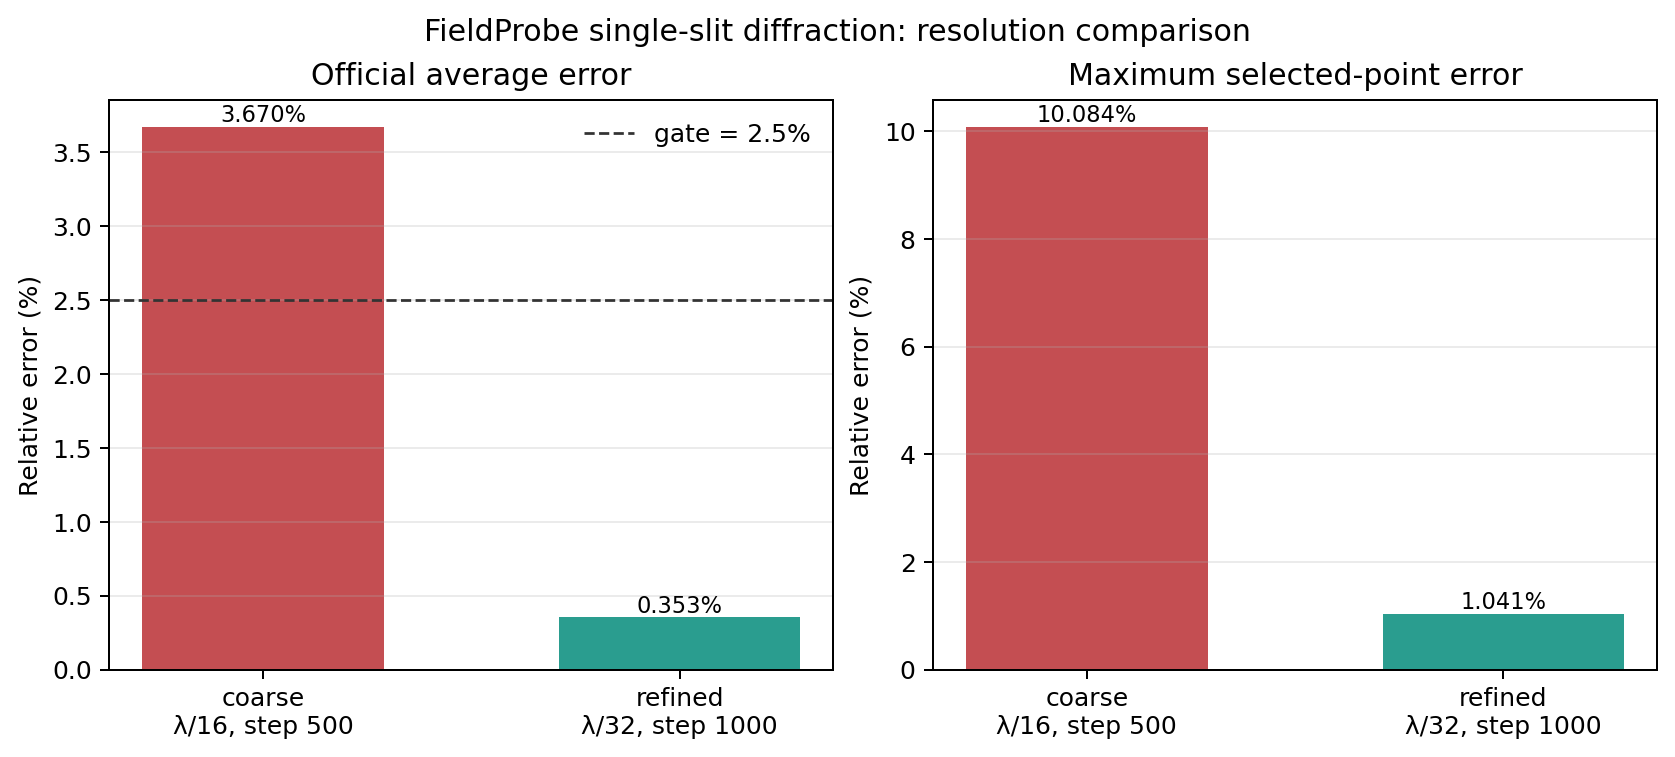
\includegraphics[width=0.8\linewidth]{../assets/figures/field-probe-resolution-comparison.png}
\end{figure}

图 8-3 由同一组 \cpath{FieldProbe} 输出的 reader-side 比较重建。

同一层里，官方测试树中还有两组更偏束流诊断的强 regression。\cpath{Examples/Tests/collider\_relevant\_diags/} 不是普通 reduced-output 烟雾测试，而是把 \cpath{ColliderRelevant} 与 \cpath{ParticleExtrema} 并排打开，然后用解析粒子样本逐项核对 \cpath{chi\_min/max/ave}、\cpath{theta\_x/theta\_y} 的 min/ave/max/std，再从 full openPMD 的 \cpath{rho\_beam\_e/rho\_beam\_p} 重建 \cpath{dL/dt} 与 reduced output 交叉验证。也就是说，这组例子验证的不是“表格写出来了”，而是 collider-oriented reduced quantities 的定义和聚合合同本身。

\cpath{Examples/Tests/diff\_lumi\_diag/} 则把 reduced diagnostics 进一步推进到带解析谱对照的束流物理量：一维 \cpath{DifferentialLuminosity} 文本表和二维 \cpath{DifferentialLuminosity2D} openPMD 网格同时输出，analysis 直接构造两束高斯束流对撞的解析 \cpath{dL/dE} 与 \codeesc{d\textasciicircum{}2L/dE\_1dE\_2}，再分别比较 1D/2D diagnostics。对本章来说，这组例子非常有价值，因为它把“reduced diagnostics 可以是纯文本列，也可以是 openPMD 网格”这件事，用同一个物理 benchmark 明确落地了。

与之相邻、但等级更弱的一组是 \cpath{Examples/Physics\_applications/beam\_beam\_collision/}。这组例子同样使用 collider 场景、Quantum Synchrotron、Breit-Wheeler、\cpath{ColliderRelevant} 与 \cpath{ParticleNumber} reduced diagnostics，但当前活跃 regression 只有 \cpath{analysis\_default\_regression.py} 提供 checksum，没有独立 \cpath{analysis.py}。因此它更准确地是一个 collider-QED application baseline：验证 relativistic electrostatic self-field、beamstrahlung、coherent pair generation 和 reduced diagnostics 的联合工作流能否稳定接通，而不是对 luminosity 谱或 Yakimenko 2019 结果做强物理断言。目录里的 \cpath{plot\_fields.py} 和 \cpath{plot\_reduced.py} 也只是说明用户应如何可视化 \code{|E|/|B|}、次级对密度、每个 beam particle 的 photon 数与 NLBW pair 数；它们不应被当成 regression analysis。

\cpath{Examples/Tests/reduced\_diags/} 本体当前则应再拆成两棵验证树。\cpath{test\_3d\_reduced\_diags} 走 \cpath{analysis\_reduced\_diags\_impl.py}：它不是只看 reduced text 文件能不能写出来，而是从 full plotfile 重新计算 \cpath{FieldEnergy}、\cpath{ParticleEnergy}、\cpath{FieldMomentum}、\cpath{ParticleMomentum}、\cpath{FieldMaximum}、\cpath{RhoMaximum} 和 parser 驱动的 \cpath{FieldReduction}，再与 \cpath{EF/EP/PF/PP/MF/MR/NP/FR\_*/Edotj.txt} 逐项对照。除 field energy 因 staggered-vs-cell-centered 差异放宽到 \cpath{0.3} 之外，其余量默认要求 \cpath{1e-12}。因此这条 regression 真正验证的是 compact observable 的物理定义和 full-state reference 一致性。

与之并列的 \cpath{test\_3d\_reduced\_diags\_load\_balance\_costs\_*} 则完全不是物理场解对照。\cpath{analysis\_reduced\_diags\_load\_balance\_costs.py} 根本不读 plotfile，而是直接从 \cpath{LBC.txt} 重建每个 rank 的总成本，再只断言 load balance 前后的效率满足 \code{efficiency_before < efficiency_after}。因此这组 tests 真正验证的是 \cpath{LoadBalanceCosts} 是否把并行运行态忠实暴露给 reduced output，而不是某个固定电磁场或粒子分布是否被精确重现。

这里还要特别写清两个边界。第一，\cpath{test\_3d\_reduced\_diags\_load\_balance\_costs\_timers\_psatd} 这个名字并没有真的把 solver 切到 \cpath{psatd}；它的 input 仍然只是 \code{inputs_base_3d + algo.load_balance_costs_update = Timers}。第二，\cpath{test\_3d\_reduced\_diags\_single\_precision} 也只看到 \cpath{analysis\_reduced\_diags\_impl.py} 里预留了 \cpath{single\_precision=True} 的放宽容差代码路径，但没有看到 active CMake test/input。因此这两条都不能被夸大成活跃的强 regression。

这一层补上以后，第 8 章里 diagnostics 的主线已经不只是“有哪些类”，而是能同时回答：

\begin{enumerate}
\item 这个 diagnostics 对象属于哪条计算主线；
\item flush 时走哪种 writer；
\item 最终落盘的是 diagnostics 视图、标准化交换格式，还是 restart 运行态。
\end{enumerate}

如果进一步按“落盘后怎么读”来分，这三类 writer 也已经形成稳定分工。\cpath{plotfile} 典型目录是：

% <-- fenced code (text)
\begin{codeblock}
diag1NNNNNN/
  Header
  Level_*/
  <species>/
  warpx_job_info
  WarpXHeader
  raw_fields/   # optional
\end{codeblock}

主读取工具是 \cpath{yt}，WarpX 文档里的标准入口就是：

% <-- fenced code (python)
\begin{codeblock}
import yt
ds = yt.load('./diags/plotfiles/plt00000/')
\end{codeblock}

如果只是要常规 field/particle 分析、AMR-aware 后处理，plotfile + yt 仍然是最顺手的默认组合。只有当打开 \code{plot_raw_fields = 1} 想看原始 staggered 网格时，才需要额外走 \cpath{Tools/PostProcessing/read\_raw\_data.py} 这条 raw reader。

\cpath{openPMD} 的目录则更扁平，典型是：

% <-- fenced code (text)
\begin{codeblock}
diag1/
  paraview.pmd
  openpmd_%06T.h5|bp5|bp4|json
\end{codeblock}

fields/particles 的层级主要在文件内部，而不是目录树展开。读者侧主工具是：

\begin{itemize}
\item \cpath{openPMD-viewer}
\item \cpath{openPMD-api}
\end{itemize}

前者适合快速浏览和 Jupyter 交互，后者适合保留完整 metadata、做并行/chunk 读取以及与外部数据生态对接。文档还专门提醒：\cpath{yt} 也能读一部分 openPMD HDF5，但没有 mesh refinement 支持，因此不能把它当成 plotfile 读法的完全替代。

\cpath{checkpoint} 则根本不是“分析目录”，而是 WarpX 自己的 restart contract。其目录会更像：

% <-- fenced code (text)
\begin{codeblock}
chkNNNNNN/
  WarpXHeader
  warpx_job_info
  Level_*/
  <species>/
  <lasers>/
\end{codeblock}

里面包含的是 \cpath{E/B} 主寄存器、\cpath{current}、coarse patch、PML、完整 species 和 lasers，以及 distribution mapping 和 reduced diagnostics checkpoint state。它的首要读取者不是 Python 数据分析工具，而是：

% <-- fenced code (text)
\begin{codeblock}
amr.restart = "../.../chk000XXX"
\end{codeblock}

也就是说，checkpoint 的主用途是“接着跑”和“恢复”，不是“直接分析”。这一点和 plotfile/openPMD 必须明确分开。

因此，对输出格式的选择可以直接收敛成三条经验：

\begin{enumerate}
\item 想做常规物理分析，优先 \cpath{plotfile}。
\item 想做标准化交换、粒子上附加场、RZ mode 或 richer metadata，优先 \cpath{openPMD}。
\item 想保留完整运行态并支持 restart，只能用 \cpath{checkpoint}。
\end{enumerate}

\cpath{restart/} 目录里还有两条很窄但很有代表性的 PICMI regression，把这三条经验压到了更细的接口层。\cpath{inputs\_test\_2d\_id\_cpu\_read\_picmi.py} 虽然也挂了 checkpoint 组件，但当前强断言其实是脚本内直接读取 \code{pti["idcpu"]} 并用 \cpath{unpack\_ids/unpack\_cpus} 验证粒子标识解包合同；\cpath{inputs\_test\_2d\_runtime\_components\_picmi.py} 则把 \cpath{picmi.Checkpoint(...)}、\cpath{amr.restart=...} 参数解析和动态 \cpath{newPid} runtime component 放在一起，证明 checkpoint front-end 接线与 runtime-attribute 写入合同可以共存，但对应的 \cpath{test\_2d\_runtime\_components\_picmi\_restart} 仍是 \cpath{FIXME} scaffold。这说明 checkpoint/PICMI 这条线已经有最小 regression 证明“前端能接上”，但还没有把“restart 后动态 runtime attrs 仍完全一致”升级成活跃强断言。

\cpath{BackTransformed} diagnostics 还有一条很值得保留的 RZ 强基准：\cpath{Examples/Tests/btd\_rz/}。它不是只检查 RZ BTD 目录结构，而是从 \cpath{back\_rz} openPMD 文件读取 back-transformed 轴上场剖面，直接拟合 boosted-frame Gaussian laser 还原到 lab frame 后的振幅、波长、包络持续时间和相位中心。因此这组例子说明：RZ \cpath{BackTransformed} diagnostics 已经不仅有 writer 合同，还有明确的物理重建合同。

checkpoint/restart 这条线也有两类很值得区分的最小基准。\cpath{test\_3d\_acceleration} / \cpath{test\_3d\_acceleration\_restart} 是最严格的一类：analysis 逐字段比较 restart 与非 restart plotfile，要求最大相对误差低于 \cpath{1e-12}，因此它真正验证的是 acceleration 基线上的 restart 可重复性，而不是某个独立“加速物理”现象。\cpath{test\_3d\_eb\_picmi} 则更像一条前端 scaffold：它把 PICMI、embedded boundary、checkpoint 与 \cpath{amr.restart=...} 放进同一个最小脚本中，但当前活跃 test 仍主要依赖 checksum，显式 restart 变体还停在 \cpath{FIXME}。因此这条线目前证明的是“EB + PICMI + checkpoint 配线能接上”，而不是“EB restart 后所有状态都已有独立强断言覆盖”。

这条 \cpath{restart\_eb} 边界还需要再强调一层：目录里虽然已经放着 \cpath{analysis\_default\_restart.py}，而且注释掉的 \cpath{test\_3d\_eb\_picmi\_restart} 也明确准备好了

% <-- fenced code (text)
\begin{codeblock}
amr.restart = "../test_3d_eb_picmi/diags/chk000030"
\end{codeblock}

与逐字段 restart 对照的调用方式，但当前活跃注册仍只有 \cpath{test\_3d\_eb\_picmi} 本体，且 \code{analysis = OFF}。因此在正文里更准确的说法应是：

\begin{enumerate}
\item \cpath{restart\_eb} 已经有完整的“未来强 restart regression”脚手架；
\item 当前活跃 CI 仍只证明 EB + PICMI + checkpoint 输出链稳定；
\item 还不能把这条线表述成“EB restart 已完成 field-level reproducibility 验证”。
\end{enumerate}

同一个 \cpath{restart/} 目录里还有一条更细、但很容易被误归到“纯 PSATD benchmark”的分支：\cpath{test\_3d\_acceleration\_psatd*}。这些输入并不是单独拿出来验证谱色散关系，而是把同一条 3D boosted acceleration workflow 切到：

\begin{itemize}
\item \code{algo.maxwell_solver = psatd}
\item \code{psatd.use_default_v_galilean = 1}
\end{itemize}

并在另一支里再额外打开：

\begin{itemize}
\item \code{psatd.do_time_averaging = 1}
\end{itemize}

然后继续复用同一个 \cpath{analysis\_default\_restart.py} 做逐字段 restart 对照。也就是说，这几条回归真正证明的是：

\begin{enumerate}
\item PSATD + Galilean acceleration workflow 的 checkpoint/restart 可重复性；
\item time-averaged PSATD update 打开后，同一 workflow 的 restart 可重复性。
\end{enumerate}

它们不是新的色散理论强基准，而是“更复杂 solver path 仍能完整写盘并无漂移恢复”的 diagnostics/restart 合同。

\section{\texttt{BoundaryScrapingDiagnostics} 与 Python scraped-particle buffer}

边界诊断是这一章里一个容易误解的特殊分支。它不是普通 full diagnostics 的“少画几列字段”，而是单独的 \cpath{diag\_type=BoundaryScraping}。

\cpath{MultiDiagnostics.cpp} 读到这个 \cpath{diag\_type} 时，会直接构造：

% <-- fenced code (cpp)
\begin{codeblock}
alldiags[i] = std::make_unique<BoundaryScrapingDiagnostics>(i, diags_names[i], diags_types[i]);
\end{codeblock}

而 \cpath{BoundaryScrapingDiagnostics::ReadParameters()} 又立刻把默认 field 输出关掉：

% <-- fenced code (cpp)
\begin{codeblock}
m_varnames_fields = {};
m_varnames = {};
m_num_buffers = AMREX_SPACEDIM*2;
if (eb_enabled) { m_num_buffers += 1; }
\end{codeblock}

这说明它的输出对象不是普通场变量，而是每个边界各自那份 \cpath{ParticleBoundaryBuffer}。

进一步看 \cpath{InitializeParticleBuffer()}，它对每个 species、每个 boundary 都直接取：

% <-- fenced code (cpp)
\begin{codeblock}
WarpXParticleContainer::Base* bnd_buffer =
    particle_buffer.getParticleBufferPointer(species_name, i_buffer);
m_output_species[i_buffer].push_back(ParticleDiag(m_diag_name, species_name, pc, bnd_buffer));
\end{codeblock}

所以 \cpath{BoundaryScrapingDiagnostics} 不是重新扫主粒子容器，而是直接消费前面边界处理阶段已经收集好的 scraped event。

这个 diagnostics 目前还有两个硬边界：

\begin{itemize}
\item 必须编译 openPMD；
\item \cpath{<diag>.format} 必须是 \cpath{openpmd}。
\end{itemize}

写出时，\cpath{Flush(i\_buffer)} 会把每个边界单独写到：

% <-- fenced code (cpp)
\begin{codeblock}
const std::string file_prefix =
    m_file_prefix + "/particles_at_" + particle_buffer.boundaryName(i_buffer);
\end{codeblock}

因此目录天然会分成 \cpath{particles\_at\_xlo}、\cpath{particles\_at\_zhi}、\cpath{particles\_at\_eb} 等子目录。更关键的是，写完后它立即：

% <-- fenced code (cpp)
\begin{codeblock}
particle_buffer.clearParticles(i_buffer);
\end{codeblock}

也就是说，\cpath{BoundaryScrapingDiagnostics} 对 \cpath{ParticleBoundaryBuffer} 是“写出并消费”的语义，而不是只读观察。

Python 接口走的是同一份底层状态。\cpath{Source/Python/WarpX.cpp} 只是把 WarpX 单例里的：

% <-- fenced code (cpp)
\begin{codeblock}
wx.GetParticleBoundaryBuffer()
\end{codeblock}

直接暴露给 \cpath{sim.extension.get\_particle\_boundary\_buffer()}。高层 \cpath{ParticleBoundaryBufferWrapper} 再把它封成：

\begin{itemize}
\item \cpath{get\_particle\_boundary\_buffer\_size(...)}
\item \cpath{get\_particle\_boundary\_buffer(...)}
\item \cpath{get\_particle\_scraped\_this\_step(...)}
\item \cpath{clear\_buffer()}
\end{itemize}

其中 \cpath{get\_particle\_scraped\_this\_step()} 并不是单独的“本步队列”，它只是用 \code{stepScraped == getistep(level)} 对累计 buffer 做一次筛选。官方 Python 文档也明确要求用户手动 \cpath{clear\_buffer()}，否则内存会持续增长。

因此，边界 scraped particle 的消费侧必须记住三个事实：

\begin{enumerate}
\item \cpath{BoundaryScrapingDiagnostics} 只写粒子，不写场，而且当前只支持 openPMD。
\item Python wrapper 和 diagnostics 共用同一个 \cpath{ParticleBoundaryBuffer}，不是两份独立副本。
\item diagnostics flush 后会自动清空对应 boundary buffer；Python 路径则需要用户自己清空。
\end{enumerate}

这一点对二次发射、探测器统计和边界通量诊断尤其关键，因为它决定了“什么时候读到哪些粒子”，本质上取决于 buffer 的消费时机，而不只是取决于边界物理本身。

\section{固定模板案例页}

为了避免 diagnostics 章节一直停留在“原理说明”，现在把四类最常用输出都压成同一模板：

\begin{enumerate}
\item 最小输入片段。
\item 典型目录树。
\item 读取入口。
\item 适用场景。
\end{enumerate}

\subsection{模板 A：\texttt{plotfile}}

\sourceline{最小输入片段}{}

% <-- fenced code (text)
\begin{codeblock}
diagnostics.diags_names = diag1

diag1.diag_type = Full
diag1.intervals = 10
diag1.fields_to_plot = Ex Ey Ez Bx By Bz rho
diag1.write_species = 1
\end{codeblock}

\sourceline{典型目录树}{}

% <-- fenced code (text)
\begin{codeblock}
diags/diag1/
  diag1000000/
    Header
    Level_0/
    <species>/
    warpx_job_info
    WarpXHeader
    raw_fields/   # optional
\end{codeblock}

\sourceline{读取入口}{}

% <-- fenced code (python)
\begin{codeblock}
import yt
ds = yt.load("./diags/diag1/diag1000000/")
\end{codeblock}

\sourceline{适用场景}{}

\begin{itemize}
\item 常规 field/particle 分析。
\item 需要 \cpath{yt} 的 AMR-aware 工作流。
\item 需要额外读取 \cpath{raw\_fields/} 做 staggered-grid 调试。
\end{itemize}

\subsection{模板 B：\texttt{openPMD}}

\sourceline{最小输入片段}{}

% <-- fenced code (text)
\begin{codeblock}
diagnostics.diags_names = diag1

diag1.diag_type = Full
diag1.format = openpmd
diag1.openpmd_backend = h5
diag1.intervals = 10
diag1.fields_to_plot = Ex Ey Ez Bx By Bz rho
diag1.write_species = 1
\end{codeblock}

如果需要 writer 阶段再把场 gather 到粒子：

% <-- fenced code (text)
\begin{codeblock}
diag1.plot_phi = 1
diag1.plot_E = 1
diag1.plot_B = 1
\end{codeblock}

\sourceline{典型目录树}{}

% <-- fenced code (text)
\begin{codeblock}
diags/diag1/
  paraview.pmd
  openpmd_000000.h5
  openpmd_000010.h5
\end{codeblock}

\sourceline{读取入口}{}

% <-- fenced code (python)
\begin{codeblock}
from openpmd_viewer import OpenPMDTimeSeries
ts = OpenPMDTimeSeries("./diags/diag1/")
\end{codeblock}

\sourceline{适用场景}{}

\begin{itemize}
\item 标准化数据交换。
\item richer metadata 或 openPMD 生态工具链。
\item full diagnostics 下的 \cpath{phi} / \cpath{E} / \cpath{B} on particles。
\end{itemize}

\subsection{模板 C：\texttt{checkpoint}}

\sourceline{最小输入片段}{}

% <-- fenced code (text)
\begin{codeblock}
diagnostics.diags_names = chk

chk.diag_type = Full
chk.format = checkpoint
chk.intervals = 100
\end{codeblock}

重启入口：

% <-- fenced code (text)
\begin{codeblock}
amr.restart = ./diags/chk/chk000100
\end{codeblock}

\sourceline{典型目录树}{}

% <-- fenced code (text)
\begin{codeblock}
diags/chk/
  chk000100/
    WarpXHeader
    warpx_job_info
    Level_0/
    <species>/
    <lasers>/
\end{codeblock}

\sourceline{读取入口}{}

首要读取者不是 Python，而是 WarpX 本体的 restart。

\sourceline{适用场景}{}

\begin{itemize}
\item 中断后续跑。
\item 完整运行态持久化。
\item reduced diagnostics 的 checkpoint state 恢复。
\end{itemize}

\subsection{模板 D：\texttt{BoundaryScraping/openPMD}}

最清楚的官方骨架来自 \cpath{thomson\_parabola\_spectrometer}：

% <-- fenced code (text)
\begin{codeblock}
diagnostics.diags_names = screen

screen.diag_type = BoundaryScraping
screen.format = openpmd
screen.intervals = 1

hydrogen1_1.save_particles_at_zhi = 1
carbon12_6.save_particles_at_zhi = 1
carbon12_4.save_particles_at_zhi = 1
\end{codeblock}

\sourceline{典型目录树}{}

% <-- fenced code (text)
\begin{codeblock}
diags/screen/
  particles_at_zhi/
    paraview.pmd
    openpmd_000001.h5
    openpmd_000002.h5
    ...
\end{codeblock}

如果是 embedded boundary scraping，则目录会变成 \cpath{particles\_at\_eb/}。

\sourceline{读取入口}{}

% <-- fenced code (python)
\begin{codeblock}
from openpmd_viewer import OpenPMDTimeSeries
series = OpenPMDTimeSeries("./diags/screen/particles_at_zhi/")
\end{codeblock}

\cpath{point\_of\_contact\_eb/analysis.py} 也用同一路径读取：

% <-- fenced code (python)
\begin{codeblock}
ts_scraping = OpenPMDTimeSeries("./diags/diag2/particles_at_eb/")
\end{codeblock}

\sourceline{适用场景}{}

\begin{itemize}
\item 探测器或屏幕 hit 记录。
\item 吸收边界通量统计。
\item EB 接触点位置和法向验证。
\item 需要把 scraped particles 落成持久文件而不是只在 Python callback 里临时消费。
\end{itemize}

和前三类相比，这一类还要额外记住：

\begin{enumerate}
\item 只支持 \cpath{openPMD}。
\item 只写粒子，不写场。
\item species 必须先开 \cpath{save\_particles\_at\_xlo/.../eb}。
\item writer filter 在 flush 时生效，因此 \cpath{plot\_filter\_function} 里的 \cpath{t} 是写出时间，不是撞边界时间。
\end{enumerate}

\cpath{thomson\_parabola\_spectrometer} 还需要再往前走一步理解。它不只是 \cpath{BoundaryScraping/openPMD} 的模板例子，也是 active 强 analysis：\cpath{CMakeLists.txt} 同时运行 \cpath{analysis.py} 和 checksum helper。\cpath{analysis.py} 会从 \cpath{screen/particles\_at\_zhi/} 读取 detector hits，再从 \cpath{diag0} 的初始 full diagnostic 读取 \cpath{uz/id/mass}，按粒子 \cpath{id} 回连出每个 detector hit 对应的初始能量，最终在 screen 平面上重建按 species 和入射能量着色的离子分离图。因此这组例子真正验证的是：

\begin{enumerate}
\item \cpath{BoundaryScraping} 在 \cpath{zhi} 屏面的 detector-hit 持久化
\item openPMD 读取链
\item \cpath{id} 跨 diagnostics 回连
\item 解析 \cpath{E\_x/B\_x} 场驱动下的 test-particle TPS optics
\end{enumerate}

所以它不应再被归到笼统的 \code{PEC / conducting boundary} 桶里。

这样整理后，第 8 章里关于 writer 的内容已经不再只是抽象分类，而是能直接给出“要什么输出，就怎么写输入、怎么找目录、怎么读文件”。

\section{Python 边界 buffer 的最小消费模板}

如果不想先把 scraped particles 写成 openPMD，而是直接在 Python 里消费 \cpath{ParticleBoundaryBuffer}，官方 examples 给出两种典型模式。

\subsection{模式 A：运行结束后统一检查}

\cpath{particle\_boundary\_scrape} 给的是最小自检骨架。species 只要打开：

% <-- fenced code (python)
\begin{codeblock}
electrons = picmi.Species(
    ...,
    warpx_save_particles_at_xhi=1,
    warpx_save_particles_at_eb=1,
)
\end{codeblock}

模拟结束后直接：

% <-- fenced code (python)
\begin{codeblock}
from pywarpx import particle_containers

particle_buffer = particle_containers.ParticleBoundaryBufferWrapper()
n = particle_buffer.get_particle_boundary_buffer_size("electrons", "eb")
weights = particle_buffer.get_particle_boundary_buffer("electrons", "eb", "w", 0)
total_weight = sum(w.sum() for w in weights)
particle_buffer.clear_buffer()
\end{codeblock}

这里有三个实现细节必须记住：

\begin{enumerate}
\item \cpath{get\_particle\_boundary\_buffer\_size()} 给的是累计到当前时刻的 scraped 数，不是本步增量。
\item \cpath{get\_particle\_boundary\_buffer()} 返回的是“每个 tile 一条数组”的列表，不会自动拼平成一块大数组。
\item Python 路径不会自动清空 buffer，必须自己 \cpath{clear\_buffer()}。
\end{enumerate}

\subsection{模式 B：callback 或在线控制里的即时事件流}

\cpath{spacecraft\_charging} 给的是“文件化 writer 和 Python 在线消费并存”的例子。它一边开：

% <-- fenced code (python)
\begin{codeblock}
part_scraping_boundary_diag = picmi.ParticleBoundaryScrapingDiagnostic(
    name="diag2",
    period=-1,
    species=[electrons, protons],
    warpx_format="openpmd",
)
\end{codeblock}

一边又在 Python 里直接读同一个 EB buffer：

% <-- fenced code (python)
\begin{codeblock}
particle_buffer = ParticleBoundaryBufferWrapper()
weights = particle_buffer.get_particle_boundary_buffer(species, "eb", "w", 0)
sum_weights_over_tiles = sum([w.sum() for w in weights])
ntot = float(mpi.COMM_WORLD.allreduce(sum_weights_over_tiles, op=mpi.SUM))
\end{codeblock}

这里它把 \cpath{period=-1} 设成只在末尾 flush 一次，目的就是在模拟中途保留完整 in-memory buffer，供 Python 侧累计计算 spacecraft 收集到的净电荷。

它的 analysis 还会继续从 full diagnostics 里抽取每个输出步的最小势值，拟合

\[
\phi(t)=v_0\left(1-e^{-t/\tau}\right),
\]

并要求拟合得到的 \cpath{v0} 和 \cpath{tau} 分别落在 \codeesc{4\%} 与 \codeesc{20\%} 的容差内。于是这组例子在第 8 章里最准确的定位就不是“演示 Python 能访问 buffer”，而是：

\begin{itemize}
\item boundary buffer 在线消费
\item Python 动态改写 EB potential
\item 以及 electrostatic diagnostics 最终能否给出正确的 charging 时间尺度
\end{itemize}

三者联动的应用级 regression。

如果逻辑只想处理“本步刚撞边界的粒子”，更直接的高层接口是：

% <-- fenced code (python)
\begin{codeblock}
weights_this_step = particle_buffer.get_particle_scraped_this_step(
    "electrons", "eb", "w", 0
)
\end{codeblock}

它本质上只是按 \code{stepScraped == current_step} 对累计 buffer 做过滤，但这已经足够支撑：

\begin{itemize}
\item secondary emission；
\item 每步边界通量统计；
\item callback 驱动的边界反应模型。
\end{itemize}

\subsection{这和 \texttt{BoundaryScrapingDiagnostics} 的分工}

现在 diagnostics 和 Python 两条路径的边界已经可以写得很清楚：

\begin{enumerate}
\item \cpath{BoundaryScrapingDiagnostics} 负责文件化持久输出，flush 后自动清空对应 boundary buffer。
\item \cpath{ParticleBoundaryBufferWrapper} 负责 Python 即时访问，默认不会自动清空。
\item 两者共用同一份 \cpath{ParticleBoundaryBuffer}，不是两份副本。
\end{enumerate}

因此，如果 diagnostics 设成频繁 flush，Python 侧看到的累计事件就会被 writer 周期性截断；如果 diagnostics 只在末尾 flush，甚至根本不开 writer，Python 才能把它当成长时间累积的事件池来用。

\section{Python field wrapper 的最小强回归}

\cpath{python\_wrappers/inputs\_test\_2d\_python\_wrappers\_picmi.py} 覆盖的是另一条 Python 接口线。它既不是粒子 callback，也不是单纯 writer smoke test，而是直接验证：

\begin{itemize}
\item \cpath{sim.fields.get(...)}
\item \cpath{MultiFabRegister}
\item valid-domain 字段
\item PML split fields
\item divergence-cleaning 标量
\end{itemize}

能否在 Python 侧被稳定访问。

这条 regression 在 \cpath{CMakeLists.txt} 里没有独立 \cpath{analysis.py}：

% <-- fenced code (cmake)
\begin{codeblock}
add_warpx_test(
    test_2d_python_wrappers_picmi
    ...
    OFF
    "analysis_default_regression.py --path diags/diag1000100"
    OFF
)
\end{codeblock}

所以如果只看 CMake，会误以为它只是 checksum-only。实际上强断言全部写在 input 脚本内部。脚本在

% <-- fenced code (python)
\begin{codeblock}
sim.initialize_inputs()
sim.initialize_warpx()
\end{codeblock}

之后，直接抓出：

% <-- fenced code (python)
\begin{codeblock}
Ex = sim.fields.get("Efield_fp", dir="x", level=0)
...
Expml = sim.fields.get("pml_E_fp", dir="x", level=0)
...
Fpml = sim.fields.get("pml_F_fp", level=0)
Gpml = sim.fields.get("pml_G_fp", level=0)
\end{codeblock}

然后给 valid domain 里的 \cpath{E/B/F/G} 填一个平滑 unit pulse，推进 \cpath{100} 步，最后不是看图片，而是逐分量检查 benchmark：

% <-- fenced code (python)
\begin{codeblock}
def check_values(benchmark, data, comp, rtol, atol):
    passed = np.allclose(
        benchmark, np.sum(np.abs(data[(), (), comp])), rtol=rtol, atol=atol
    )
    assert passed
\end{codeblock}

这里 \code{data[(), (), comp]} 的意思也很关键：

\begin{itemize}
\item \cpath{()} 取 valid + ghost 全范围；
\item \cpath{comp} 用来访问 PML split-field 的不同 component。
\end{itemize}

脚本会依次断言：

\begin{itemize}
\item \cpath{Ex/Ey/Ez}
\item \cpath{Bx/By/Bz}
\item \cpath{F/G}
\item \cpath{pml\_E\_fp}
\item \cpath{pml\_B\_fp}
\item \cpath{pml\_F\_fp}
\item \cpath{pml\_G\_fp}
\end{itemize}

的每个相关 component 都与固定 benchmark 一致，而且若干应为零的 component 也显式要求保持为零。于是这条 test 的真实定位应当是：

\begin{itemize}
\item Python field wrapper / PML split-field access
\end{itemize}

而不是过粗的 \code{Python API / callbacks}。它验证的是 \cpath{pywarpx} 经由 \cpath{MultiFabRegister} 暴露出来的非 owning \cpath{MultiFab} 视图，在 valid domain、ghost cell、PML 和 cleaning 字段这几层上都没有被包装错。

\section{MPI transport 环境注意}

某些 MPI/OFI 组合会受网络接口选择影响；在这类环境中，小规模复现实验可设置：

% <-- fenced code (bash)
\begin{consoleblock}
FI_PROVIDER=tcp
\end{consoleblock}

这不是物理参数，而是 MPI transport 的环境兼容设置。复现实验应记录环境变量、binary 版本、输入文件、输出目录和分析脚本；不要把它误当成会改变 PIC 物理模型的输入参数。

\section{Langmuir 与均匀等离子体的运行证据}

下面三项 reader-side 比较分别覆盖 Langmuir 时间采样、均匀等离子体守恒统计和二者的分析入口：

\begin{enumerate}
\item 对同一份 Langmuir 官方输入，将 \cpath{diag1/openpmd.intervals} 从 \cpath{40} 改为 \cpath{1}，运行 80 步，得到 81 个逐步快照；
\item 对 \cpath{Ez} 的目标空间模做投影，用两正交分量拟合时间频率，并逐快照计算 \cpath{divE-rho/epsilon\_0}；
\item 用 \cpath{yt} 读取 uniform-plasma 初末 plotfile，统计粒子数、粒子总权重、场能、粒子动能和总能量。
\end{enumerate}

Langmuir 的受控复现实验给出：

\begin{itemize}
\item \cpath{81} 个快照；
\item 解析 \cpath{omega\_p=1.128292045086e14}，拟合值为 \cpath{1.128697661742e14}；
\item 相对频率误差 \cpath{3.595e-4}；
\item 官方 \cpath{analysis\_1d.py} 在同一族运行上给出场最大相对误差 \cpath{1.70e-3}、最终 \cpath{divE-rho/epsilon\_0} 误差 \cpath{8.35e-12}，均通过原始阈值；
\item 逐步 reader-side 扫描的最大守恒误差为 \cpath{3.149e-10}，发生在中间快照，因此不能把“每一步都满足官方 \cpath{1e-11} 阈值”写成已验证事实。
\end{itemize}

Uniform-plasma 的受控复现实验给出：

\begin{itemize}
\item 初末粒子数均为 \cpath{65536}；
\item 粒子总权重相对变化为 \cpath{0}；
\item 初始场能量为零，所以场能相对变化率有意标记为 \code{undefined (zero baseline)}；
\item 粒子动能变化约 \codeesc{7.06\%}，总能量变化约 \codeesc{1.97\%}。
\end{itemize}

将同一输入延长到 \cpath{100} 步、每 \cpath{10} 步写出一个 plotfile 后，粒子总权重在全部 \cpath{11} 个快照中保持不变，末态总能量相对初态变化 \cpath{1.387e-2}，时间序列中的最大绝对相对偏差为 \cpath{2.518e-2}。这比单看 10 步终点更能说明短时热背景统计范围，但仍不足以构成热平衡能量守恒 gate；后者应与 \cpath{energy\_conserving\_thermal\_plasma} 的专门 analysis 绑定。

官方 2D \cpath{energy\_conserving\_thermal\_plasma} 输入运行 500 步，产生 \cpath{EF.txt} 和 \cpath{EP.txt} 六个 reduced-energy 样本；其 \cpath{analysis.py} 通过，独立 reader-side 计算同一 \cpath{EF+EP}，得到最大总能量相对漂移 \cpath{1.031e-4}，低于官方 \cpath{3.000e-3} 阈值。由此可以把两类证据明确分开：uniform-plasma 负责粒子数、I/O 和热背景 workflow 统计，energy-conserving-thermal-plasma 才负责 energy-conserving gather 的强能量漂移 gate。

同一官方 family 的 1D sibling 也在 500 步运行中通过官方 analysis，最大漂移为 \cpath{3.009e-4}。1D/2D 都使用 \cpath{EF+EP}、\cpath{0.003} 阈值和 6 个采样点，但不应把两种几何的物理轨迹误写成数值等价。

图 8-2 把 1D/2D 的 \cpath{EF+EP} 和归一化漂移放在同一张图里。左图保留不同几何的能量尺度差异，右图直接与共同的 \cpath{0.003} gate 对照；因此读者可以同时看到“能量在场能与粒子能之间交换”和“总能量误差仍被 gate 约束”这两个不同层次。

\begin{figure}[htbp]
\centering
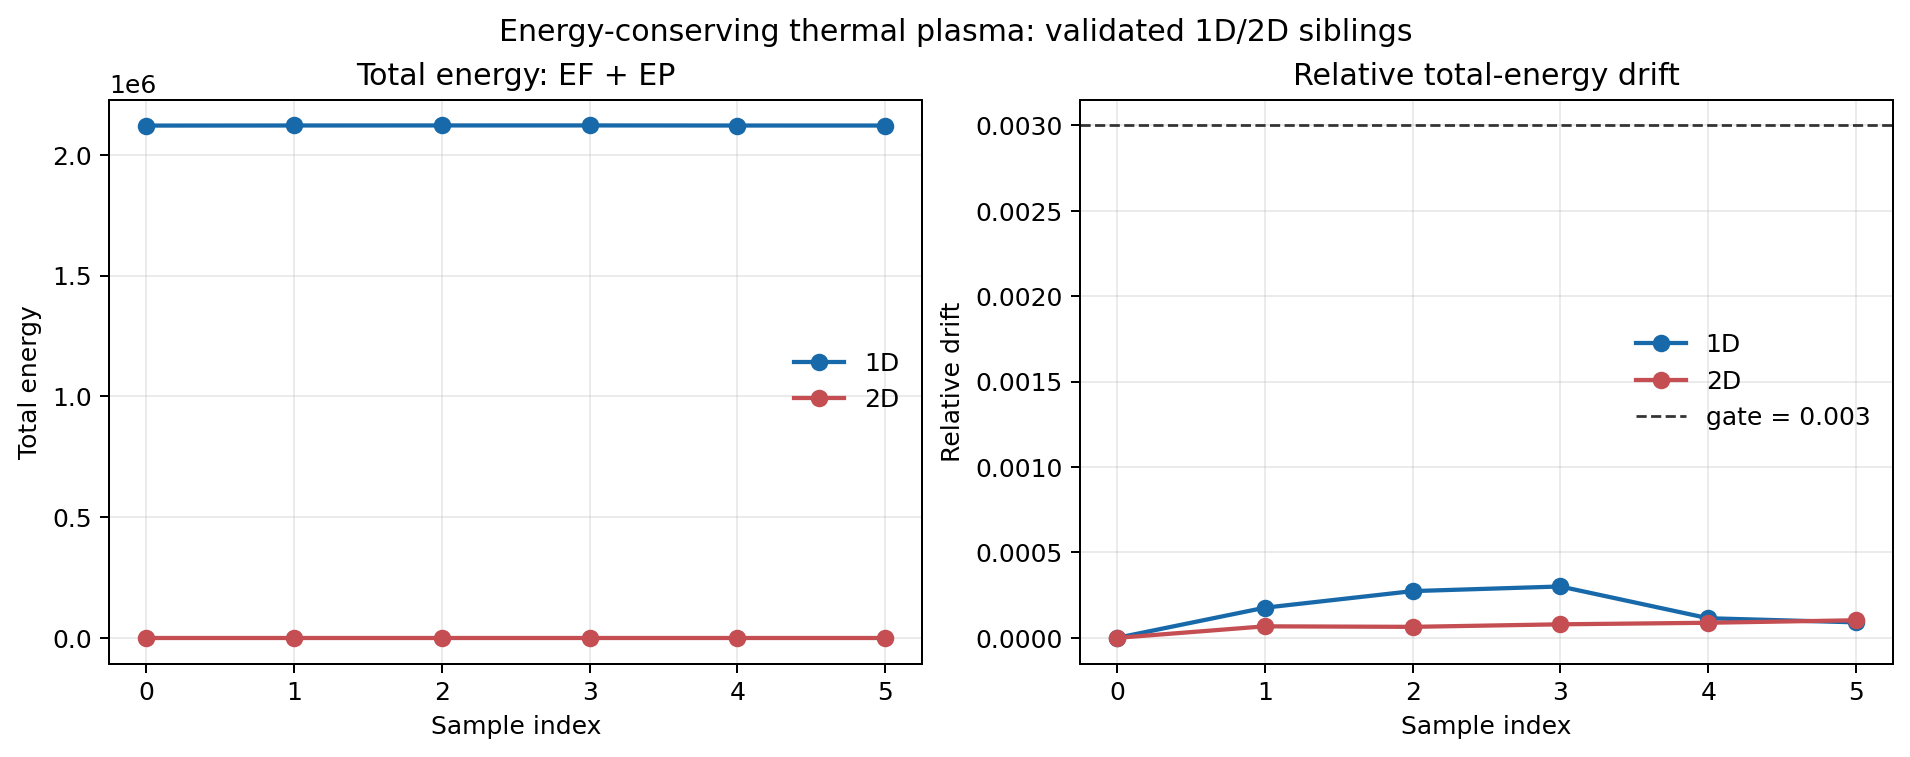
\includegraphics[width=0.8\linewidth]{../assets/figures/energy-conserving-thermal-plasma-1d-2d.png}
\end{figure}

\subsection{Reduced diagnostics 与 full-state reference 对照}

按官方 2-rank 配置执行 \cpath{Examples/Tests/reduced\_diags/inputs\_test\_3d\_reduced\_diags} 后，末态为 \cpath{diags/diag1000200}。官方 \cpath{analysis\_reduced\_diags.py} 从该 plotfile 重新计算粒子能量/动量、场能/动量、场最大值、rho 最大值、粒子数以及 \cpath{FR\_Max/FR\_Min/FR\_Integral/Edotj} 等 parser-driven \cpath{FieldReduction}，再逐项与 \cpath{EP/EF/PP/PF/MF/MR/NP/FR\_*/Edotj.txt} 对照。

共比较 60 个 reduced observable，官方 analysis 通过。除 field energy 外，最大相对误差为 \cpath{4.125e-13}；field energy 的相对误差为 \cpath{2.483e-1}，仍低于官方为 staggered Yee reduced energy 与 cell-centered plotfile reference 设置的专用 \cpath{0.3} 容差。独立 reader-side 比较给出相同的误差分层。

这条证据的准确含义是“compact reduced observable 与 full-state reference 的定义和 writer 输出一致”，不是说 60 个量都构成独立物理守恒定律。尤其 field energy 的 \codeesc{24.8\%} 误差必须保留其 staggered/cell-centered 离散表示边界，不能被误读成普通量的数值精度。

图 8-4 将这两个误差层分开画出：左图在对数尺度下显示 59 个非 field-energy observable 的排序误差，右图单独显示 staggered field-energy 的 \cpath{0.2483} 误差与 \cpath{0.3} 专用 gate。这样图表本身就保留了“普通量接近机器精度、field energy 仍有离散表示差异”的证据结构，而不是只给出一个混合最大值。

\begin{figure}[htbp]
\centering
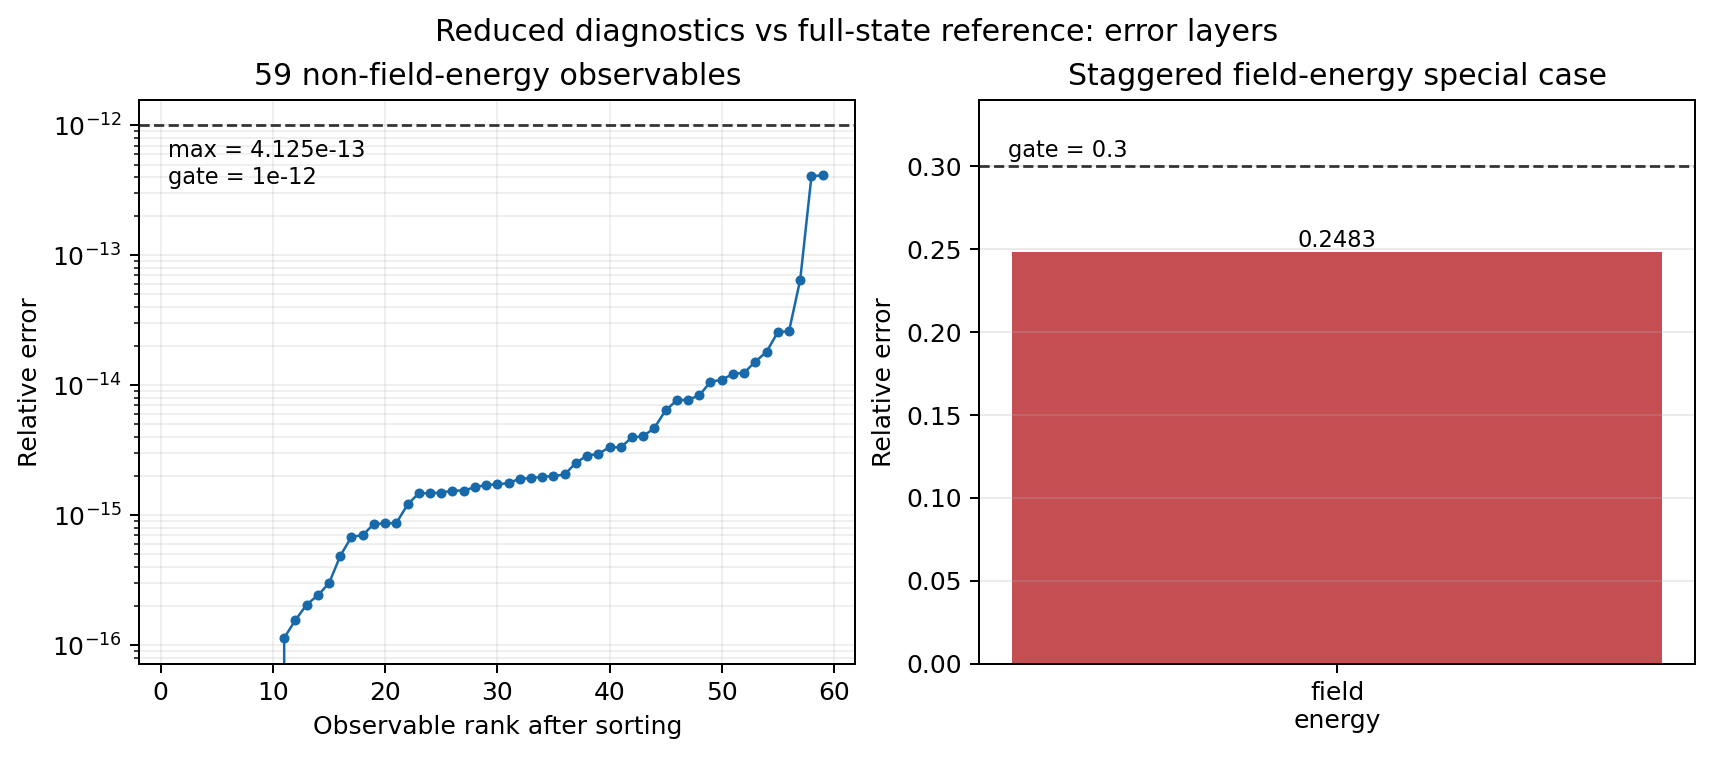
\includegraphics[width=0.8\linewidth]{../assets/figures/reduced-diags-error-layers.png}
\end{figure}

图 8-4 由同一组 reduced diagnostics 与 full-state 输出的 reader-side 比较重建。

\subsection{LoadBalanceCosts：性能诊断的 efficiency gate}

同一 \cpath{reduced\_diags} family 还包含一条不读取 plotfile 的性能诊断分支：\cpath{inputs\_base\_3d} 使用 \code{128 x 32 x 128} 网格、16 个 box、\code{algo.load_balance_intervals = 2}，并由 \cpath{LoadBalanceCosts} 将每个 box 的 cost、rank、level、几何位置和粒子数写入 \cpath{LBC.txt}。官方 analysis 按 rank 汇总 box cost，再计算

\[
\eta = \frac{1}{N_\mathrm{rank}}
\sum_r \frac{C_r}{\max_{r'} C_{r'}}.
\]

它比较第 1 行（load balance 前）与第 2 行（load balance 后），要求 \code{eta_after > eta_before}。按官方 2-rank 配置分别运行 \cpath{Heuristic} 与 \cpath{Timers} 两个 sibling：

% <-- table block (source: 08-diagnostics-cases L1532)
\begin{tabularx}{\textwidth}{LrrL}
\toprule
cost source & before & after & result \\
\midrule
\endfirsthead
\toprule
cost source & before & after & result \\
\midrule
\endhead
\cpath{Heuristic} & \cpath{0.625252} & \cpath{1.000000} & \cpath{PASS} \\
\cpath{Timers} & \cpath{0.744780} & \cpath{0.996162} & \cpath{PASS} \\
\bottomrule
\end{tabularx}

因此 \cpath{LoadBalanceCosts} 的强合同不是“有一个 LBC 文本文件”，而是它能把 box-level cost 通过 MPI 汇总成 rank-level efficiency，并观察到重分配后的效率改善；这属于性能/并行态验证，不应与 \cpath{reduced\_diags} 的 compact physical observable 对照混成同一类 gate。

图 8-6 将两条 cost source 的 rank-level efficiency 直接画成 before/after 对照。Heuristic 从 \cpath{0.625252} 提升到 \cpath{1.0}，Timers 从 \cpath{0.744780} 提升到 \cpath{0.996162}；图表表达的是负载重分配后的性能改善，不是场或粒子物理精度。

\begin{figure}[htbp]
\centering
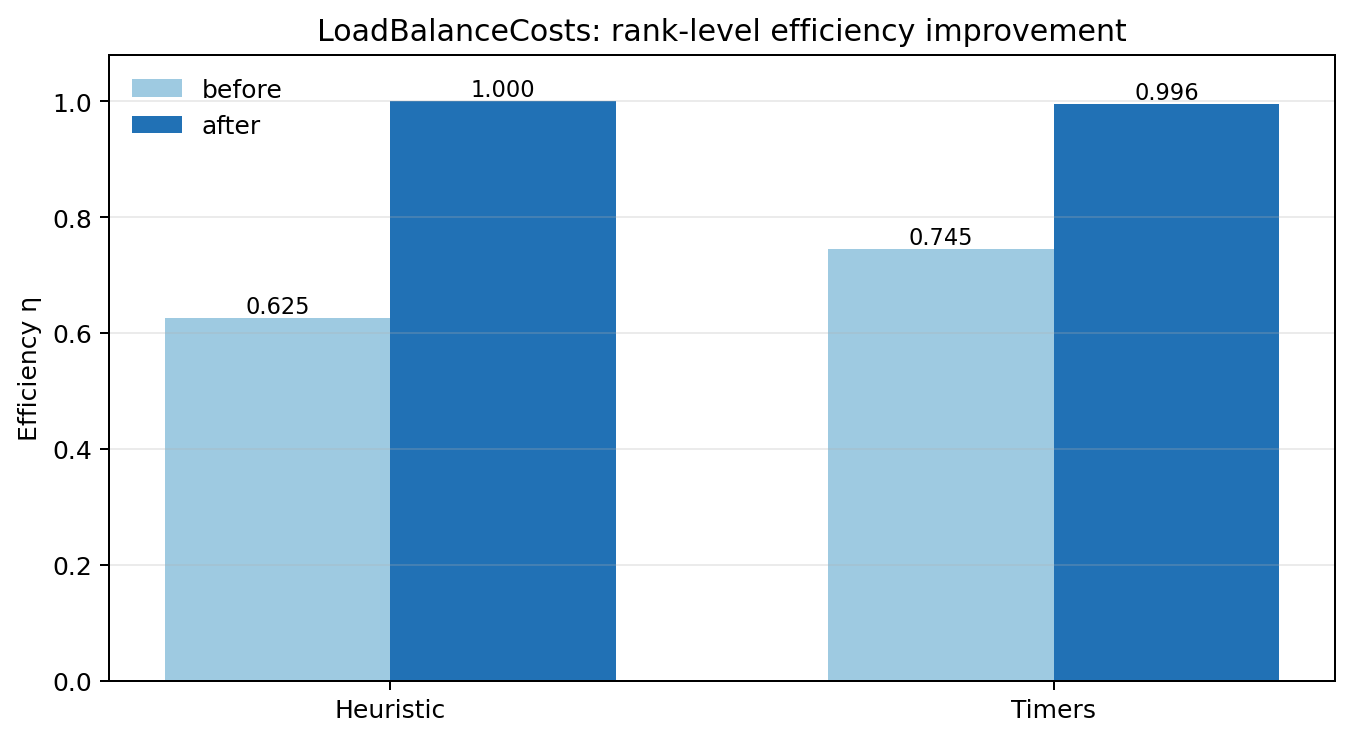
\includegraphics[width=0.8\linewidth]{../assets/figures/load-balance-efficiency.png}
\end{figure}

图 8-6 由 \cpath{LBC.txt} 的 reader-side 汇总重建。

\subsection{\texttt{ColliderRelevant}：束流统计与 luminosity-rate 聚合合同}

\cpath{Examples/Tests/collider\_relevant\_diags/} 提供了另一条强 reduced-diagnostics regression。它在同一 3D、2-rank 输入中同时输出 \cpath{ColliderRelevant\_beam\_e\_beam\_p}、\cpath{ParticleExtrema\_beam\_e/beam\_p} 和 openPMD full state。官方 \cpath{analysis.py} 使用输入中的三个解析宏粒子样本，逐项检查每个 beam 的 \cpath{chi\_min/max/ave}、位置均值/标准差和 \cpath{theta\_x/theta\_y} 的 min/ave/max/std，并把 \cpath{ParticleExtrema} 与 \cpath{ColliderRelevant} 交叉核对；随后从 \cpath{rho\_beam\_e}、\cpath{rho\_beam\_p} 和粒子电荷重建

\[
\frac{dL}{dt}=2c\,\Delta V\sum_i
\frac{\rho_{e,i}}{q_e}\frac{\rho_{p,i}}{q_p}.
\]

在两次 openPMD iteration 中，\code{dL/dt = 4.42662301265625e8}，与 reduced text 的对应两行完全一致；\cpath{ColliderRelevant} 为 2 行/33 列，两个 \cpath{ParticleExtrema} 文件各为 2 行，官方 analysis 与独立 reader-side 比较均通过。该结果验证的是 collider-oriented quantity 的定义、统计和聚合 writer 合同，不等于已经完成 \cpath{diff\_lumi\_diag} 的解析谱 benchmark，也不等于 \cpath{beam\_beam\_collision} 的 QED 应用级物理复现。

图 8-7 将两个 openPMD iteration 的 \cpath{dL/dt} 交叉结果叠加显示。两个 reader-side reconstruction 点与 \cpath{ColliderRelevant} reduced 点完全重合，且 JSON 报告给出的相对误差均为 \cpath{0}；这张图验证的是聚合定义和 writer/reader 对齐，不是 luminosity 随束流演化的独立动力学 benchmark。

\begin{figure}[htbp]
\centering
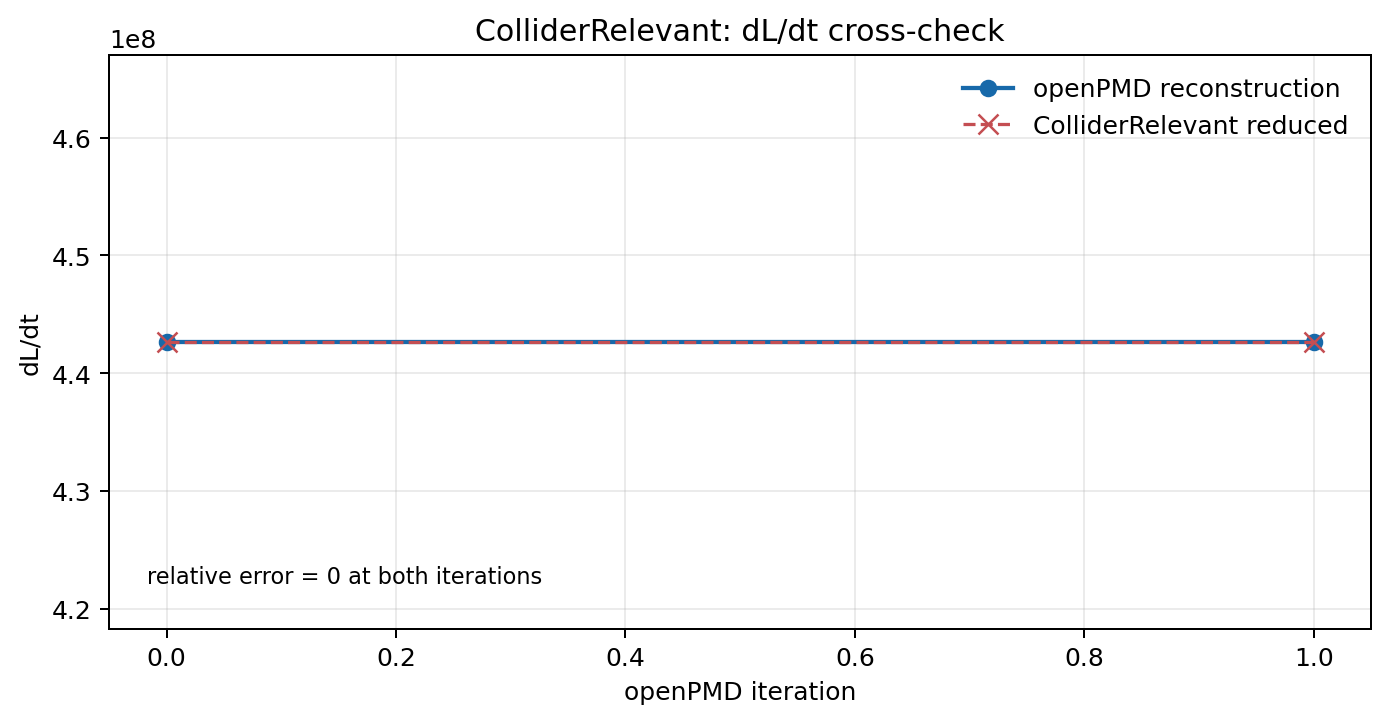
\includegraphics[width=0.8\linewidth]{../assets/figures/collider-dldt-consistency.png}
\end{figure}

图 8-7 由同一 openPMD 与 reduced-output 对照重建。

\subsection{\texttt{DifferentialLuminosity}：1D/2D 解析谱与 AMR 对照}

\cpath{Examples/Tests/diff\_lumi\_diag/} 把 reduced diagnostics 推进到能量微分 luminosity 的解析 benchmark。共享的 \cpath{inputs\_base\_3d} 设定两束相向高斯束，1D \cpath{DifferentialLuminosity} 输出总能量谱，2D \cpath{DifferentialLuminosity2D} 输出两个入射束能量的二维网格；官方 \cpath{analysis.py} 分别用高斯束解析式比较末态 1D 与 2D 结果。这个分析依赖 \cpath{openpmd\_viewer} 读取 2D openPMD series，而不是把二维数据误当作普通文本列。

按官方 2-rank 配置完成三组 sibling，三组都在 step 80 输出 128 个 1D 能量 bin 和 \code{128 x 128} 的 2D 网格：

% <-- table block (source: 08-diagnostics-cases L1568)
\begin{tabularx}{\textwidth}{LrrrL}
\toprule
case & AMR max level & 1D error / tolerance & 2D error / tolerance & result \\
\midrule
\endfirsthead
\toprule
case & AMR max level & 1D error / tolerance & 2D error / tolerance & result \\
\midrule
\endhead
leptons & 0 & \codeesc{0.8903\% / 2.0\%} & \codeesc{2.6890\% / 4.0\%} & \cpath{PASS} \\
leptons + AMR & 1 & \codeesc{0.9796\% / 2.0\%} & \codeesc{3.0042\% / 4.0\%} & \cpath{PASS} \\
photons & 0 & \codeesc{2.0119\% / 2.1\%} & \codeesc{4.9327\% / 6.0\%} & \cpath{PASS} \\
\bottomrule
\end{tabularx}

这些比较使用独立 reader-side analysis。这组结果补上了束流诊断链中的解析谱 physics gate；AMR sibling 的意义是验证中心细化区域仍能保持相同的 reduced luminosity 定义，而不是宣称 AMR 与 uniform-grid 轨迹逐点相同。

图 8-5 将三组 sibling 的 1D/2D 相对误差和各自 gate 并列展示。photons 使用报告中独立的 \codeesc{2.1\%/6.0\%} 容差，不能直接套用 leptons 的阈值；三组柱状值均低于对应虚线 gate，图表只表达解析谱误差合同，不把 reduced writer 的文件形状误写成额外物理结论。

\begin{figure}[htbp]
\centering
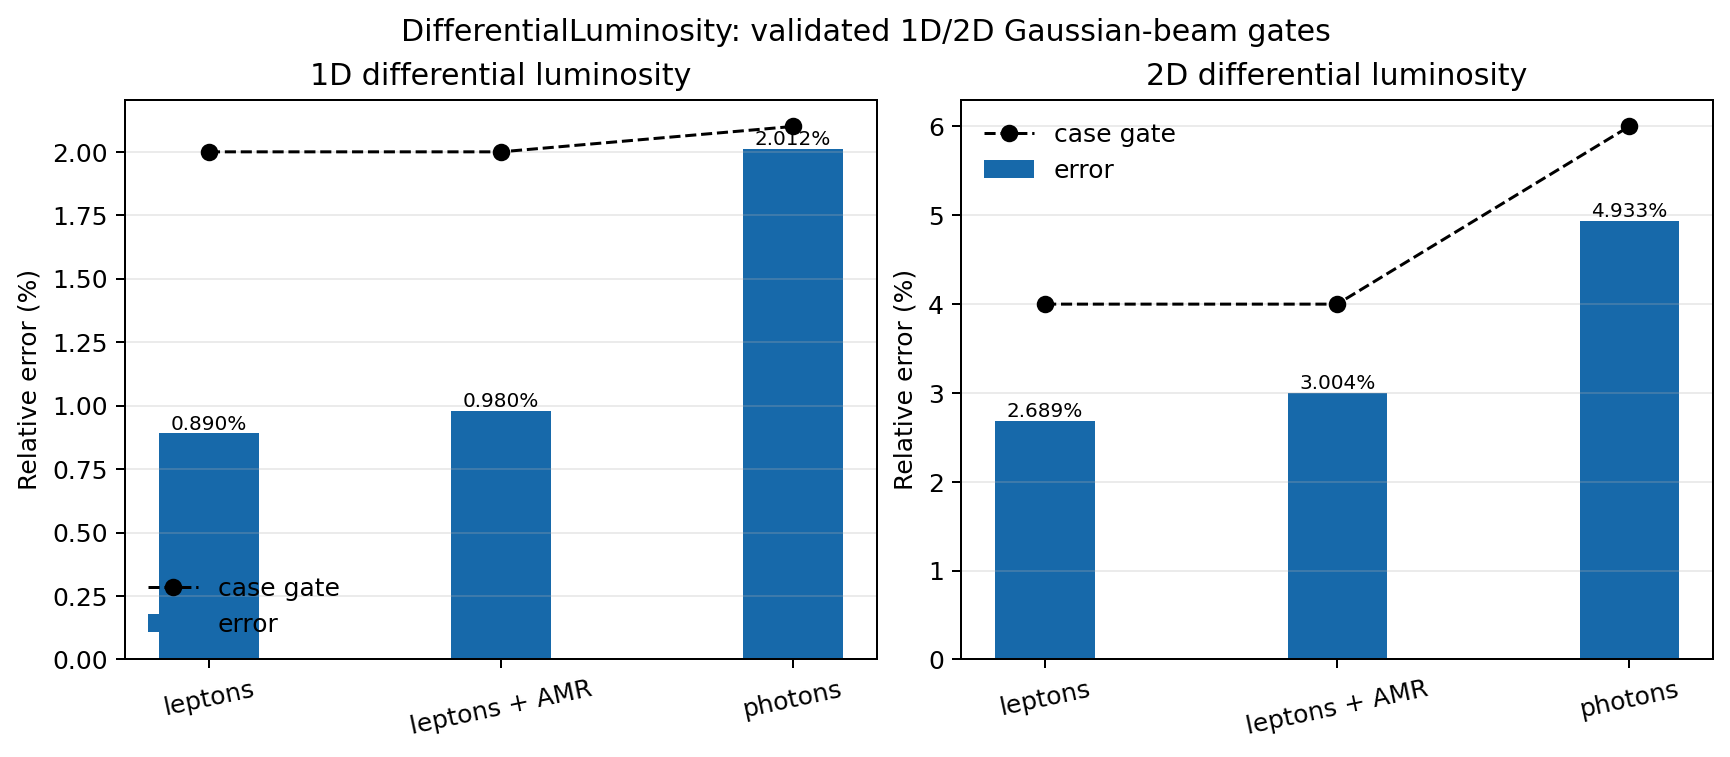
\includegraphics[width=0.8\linewidth]{../assets/figures/diff-lumi-errors.png}
\end{figure}

图 8-5 由三组解析谱比较的误差结果重建。

\subsection{\texttt{ParticleHistogram2D}：二维 openPMD writer 合同}

官方测试树目前没有单独的 \cpath{ParticleHistogram2D} CMake regression；可用 \cpath{Examples/Physics\_applications/laser\_ion/} 的官方 2-rank application 作为完整 producer。输入同时配置 \cpath{PhaseSpaceIons} 和 \cpath{PhaseSpaceElectrons} 两个二维 histogram：两者都使用 \cpath{z} 作为 abscissa、\cpath{uz} 作为 ordinate、\code{1000 x 1000} bins、\code{value_function = w}，而 electrons 还增加 \code{sqrt(x*x+y*y) < 1e-6} filter。官方 CMake analysis 只负责 time-averaged field 与 instantaneous field 的一致性，因此不能单独被写成 histogram physics gate；独立 reader-side 检查则验证 histogram series 的 writer 语义。

在受控复现实验中，两个 series 都写出 \cpath{0} 和 \cpath{100} 两个 BP5 iteration，数据形状均为 \code{1000 x 1000}，axis labels 为 \cpath{uz/z}，所有数据有限且存在非零 bin；官方 time-average analysis 通过。\cpath{PhaseSpaceIons.txt} 与 \cpath{PhaseSpaceElectrons.txt} 的大小均为 \cpath{0}，这是预期结果：\cpath{ParticleHistogram2D::WriteToFile()} 绕过基类逐行文本 writer，直接创建 \codeesc{reducedfiles/<name>/openpmd\_\%T.<backend>} series，因此空 \cpath{.txt} companion 不能被误判成 histogram 丢失。

这条证据的边界也需要保留：它证明二维 histogram 的配置、openPMD layout、轴元数据和 writer 输出链成立，不等于已经用独立解析分布证明 laser-ion phase-space 的物理收敛性；后者需要更高分辨率/粒子数以及针对相空间分布的物理参考结果。

在不改变这条边界的前提下，reader-side analysis 对 BP5 数组做加权统计。\cpath{PhaseSpaceIons} 的总权重从 iteration 0 的 \cpath{3.9975794429219594e18} 到 iteration 100 的 \cpath{3.997579442921919e18}，相对变化约 \cpath{1.0e-14}；\cpath{std(z)} 保持在 \code{1.47204e-6 m}，而 \cpath{std(uz)} 从数值零增长到 \cpath{4.78558e-4}。受径向 filter 影响的 \cpath{PhaseSpaceElectrons} 总权重从 \cpath{5.30929e17} 变为 \cpath{5.32861e17}，\cpath{std(uz)} 从 \cpath{0.196998} 变为 \cpath{0.199300}。这些统计量把“相空间图发生了什么变化”从视觉判断推进成可复现的 weighted-moment 摘要，但仍不能替代更高分辨率/粒子数的 convergence study。

随后又做了一个匹配物理时间的 producer 对照：baseline 使用 \cpath{384x512} 网格、\code{dt=1.083064693e-16 s}、100 步，refined 使用 \cpath{768x1024} 网格、\code{dt=5.415323467e-17 s}、200 步；两者最终时间差只有 \code{3.31e-29 s}。reader-side analysis 对两个 BP5 series 的总权重、\cpath{std(z)} 和 \cpath{std(uz)} 设置了 \cpath{1e-3/1e-2/5e-2} 的局部稳定性阈值，ions/electrons 均通过：\cpath{std(z)} 相对差为 \cpath{5.51e-4/2.02e-4}，\cpath{std(uz)} 相对差为 \cpath{2.04e-3/4.47e-2}。这是“网格加密后 reader-side 加权宽度仍稳定”的局部证据，不是严格的物理收敛阶证明；两套 producer 都是单进程，运行结束时的 OFI \cpath{MPI\_Finalize} 环境尾噪声不影响已写出的 BP5 数据读取。

同一比较还记录了 \cpath{1x1} particles-per-cell 的负对照。它的 ions 宽度仍接近 baseline，但 electrons 总权重相对差为 \cpath{1.9471e-3}，超过 \cpath{1e-3} 阈值，因此 \cpath{weighted\_width\_stability} 被拒绝。这个负结果应保留为低采样负对照，而不是被静默删除；高粒子数区间需要与它分开判断。

为判断该负结果是否只是单个低采样点，比较 \cpath{1x1/2x2/4x4/8x8} 四档 particles-per-cell 的相邻档位：\code{1x1 -> 2x2} 是预期负对照，\code{2x2 -> 4x4} 与 \code{4x4 -> 8x8} 是高粒子数局部稳定性 gate。electrons 总权重差依次为 \cpath{1.9471e-3}、\cpath{4.2685e-4}、\cpath{3.6534e-4}，ions/electrons 的总权重、\cpath{std(z)}、\cpath{std(uz)} 在高粒子数 pair 均通过。这支持“增加粒子数后该 reader-side 统计总体更稳定”的方向性判断，但仍是单进程、单一激光离子 case 的局部矩比较，不足以给出正式收敛阶或上游 regression gate。

图 8-8 直接从 BP5 series 读取 \cpath{PhaseSpaceIons} 与 \cpath{PhaseSpaceElectrons} 的 iteration 0/100 数据，并按每个面板的非零 bin 裁剪显示范围。它展示的是 writer 实际落盘的 \cpath{uz-z} 相空间结构和随 iteration 的变化；由于每个面板使用独立对数颜色归一化，颜色不能用于跨 species 或跨 iteration 的绝对产额比较。完整数组仍为 \code{1000 x 1000}，空 \cpath{.txt} sidecar 也仍是预期的 writer 路径边界。

\begin{figure}[htbp]
\centering
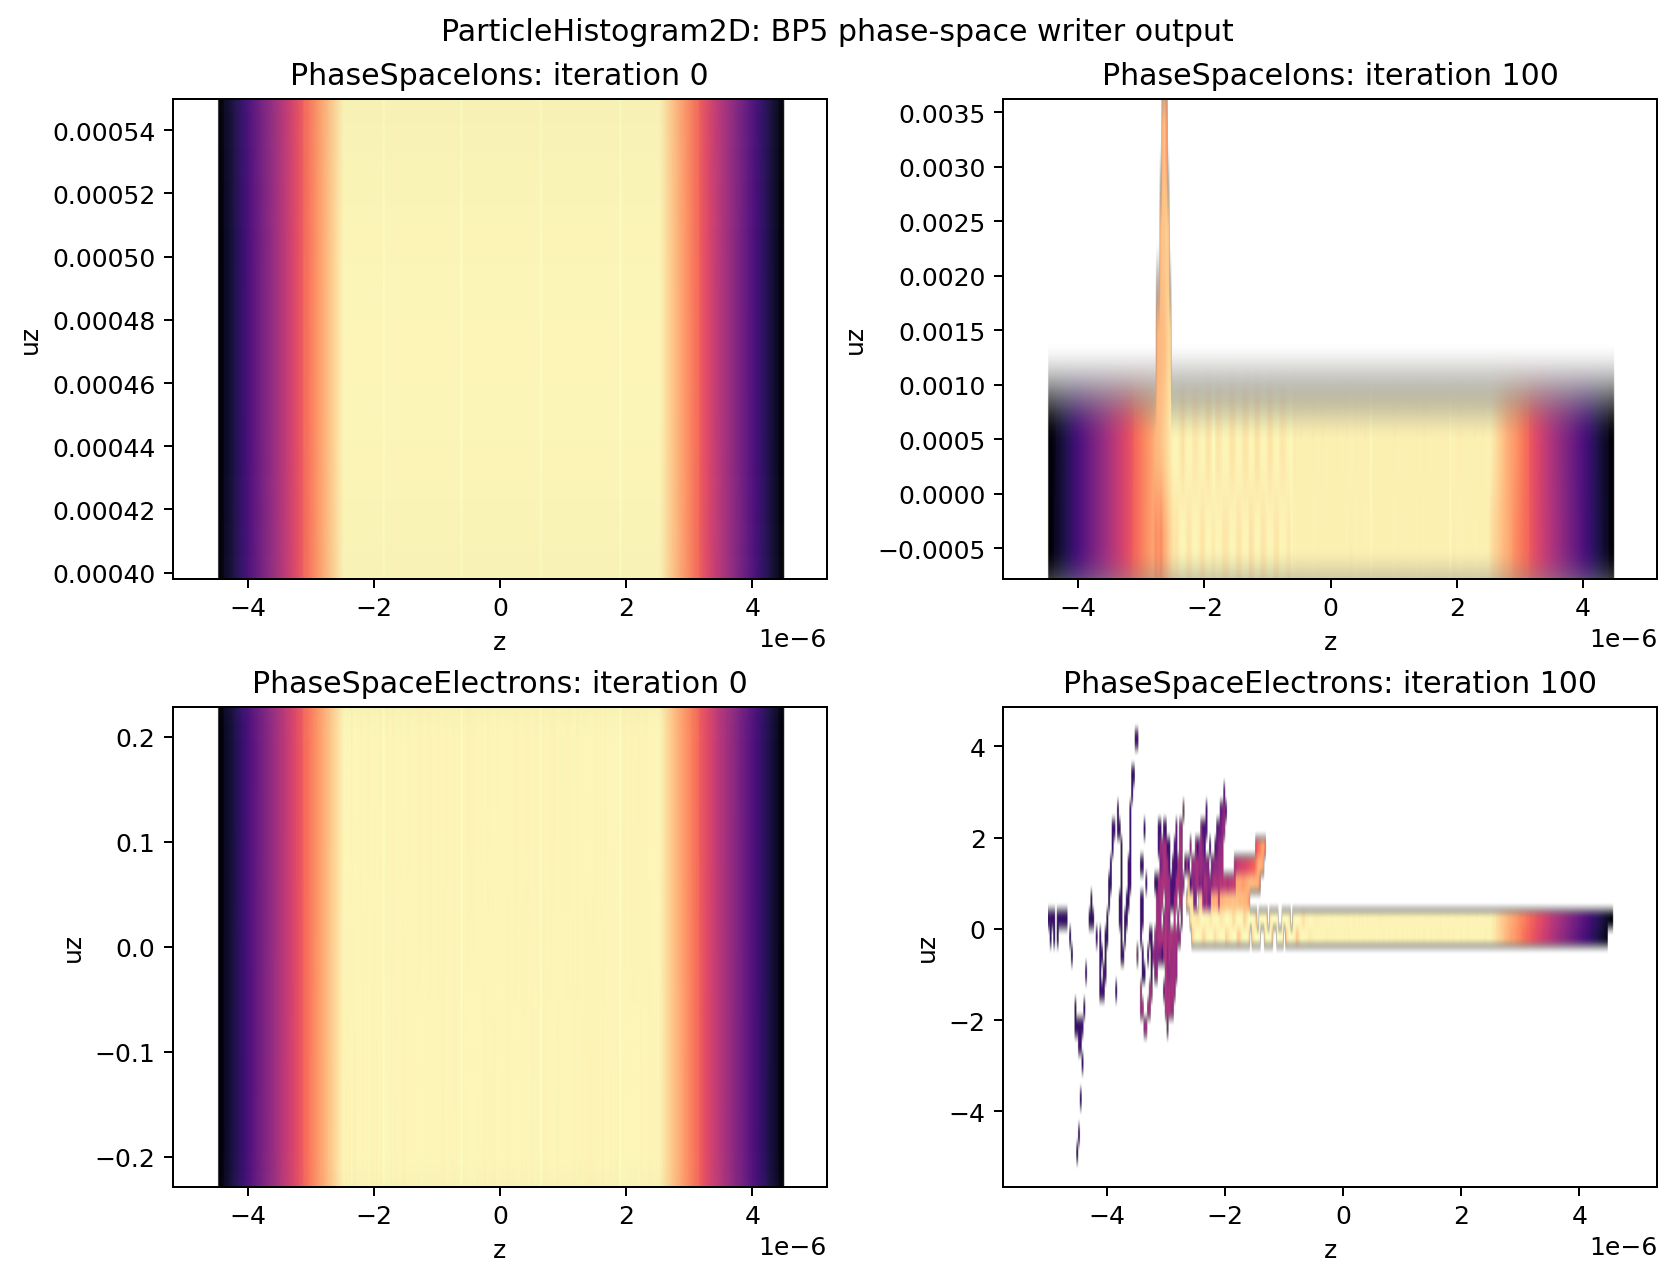
\includegraphics[width=0.8\linewidth]{../assets/figures/particle-histogram2d-phase-space.png}
\end{figure}

图 8-12 用同一份四档 pairwise contract 把粒子数敏感性归一化到各自局部 gate：虚线是 gate 边界，纵轴小于 1 表示通过。\code{1x1 -> 2x2} 的电子总权重仍越过边界，\code{2x2 -> 4x4} 和 \code{4x4 -> 8x8} 则落在边界以内；新增 trend contract 将这种“预期负对照 + 高粒子数局部通过”固定为可复查状态，但不把单一 case 的 reader-side 矩合同写成正式收敛阶。

\begin{figure}[htbp]
\centering
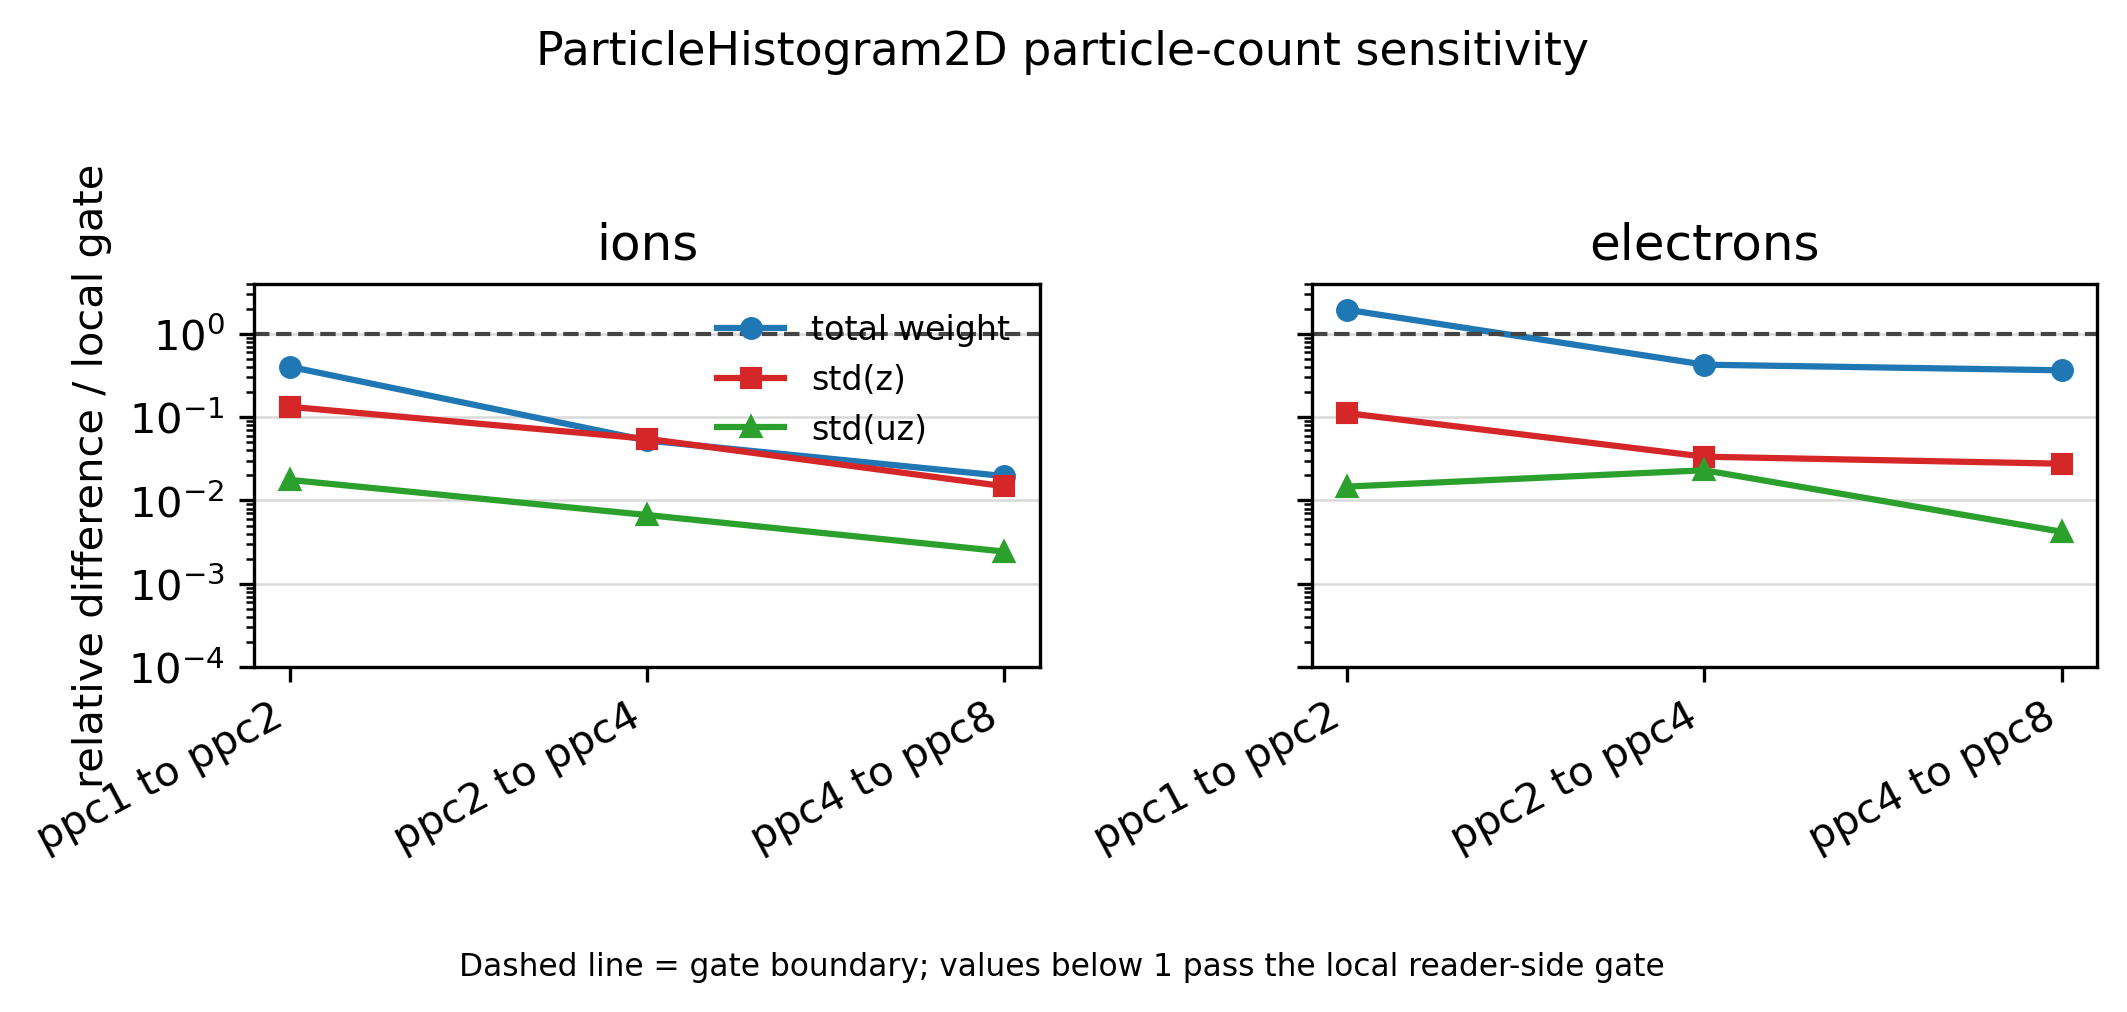
\includegraphics[width=0.8\linewidth]{../assets/figures/particle-histogram2d-particle-count.png}
\end{figure}

图 8-8 由 BP5 series 的 reader-side 读取重建。

\subsection{\texttt{BeamRelevant}：束流矩与截断高斯束合同}

\cpath{BeamRelevant} 是文本型束流诊断，和 \cpath{ColliderRelevant} 的逐粒子 \cpath{chi/theta} 统计不同。3D 路径固定输出 22 个物理量：位置与动量均值、\cpath{gamma} 均值、位置/动量/\cpath{gamma} rms、三方向 emittance、Twiss \cpath{alpha/beta} 以及总 charge；连同步列和时间列共 24 列。其实现先按粒子权重做并行归约，再从二阶矩构造 rms、emittance 和 Twiss 量，因此最小验证应同时检查 schema、权重聚合和几何分布，而不是只检查文件存在。

以官方 \cpath{initial\_distribution} 中的 \cpath{beam} 参数为基准，可以用只包含该 beam、\code{bmmntr = BeamRelevant} 的 3D、1-rank、\cpath{max\_step=0} 输入检查初始化束流矩。reader-side analysis 对 \cpath{bmmntr.txt} 的独立读取给出 1 行/24 列：\cpath{z\_cut=2} 的截断高斯束 charge 期望值为 \code{-9.544997e-21 C}，实测为 \code{-9.544980e-21 C}，相对误差 \cpath{1.77e-6}；横向 rms 为 \code{0.249884/0.249765 m}，纵向 rms 为 \code{0.220356 m}，均通过 \codeesc{2\%} gate；均值、emittance、Twiss 相关输出均有限且满足正值边界。

图 8-9 将这个初始化检查的两个主要物理量画出来：左图是实际总 charge 相对于截断高斯期望值的比值，右图是三个位置 rms 与解析目标的对照。图中没有把单行输出扩展成虚假的时间演化；gamma、emittance 和 Twiss 量仍只要求满足有限性与正值边界。

\begin{figure}[htbp]
\centering
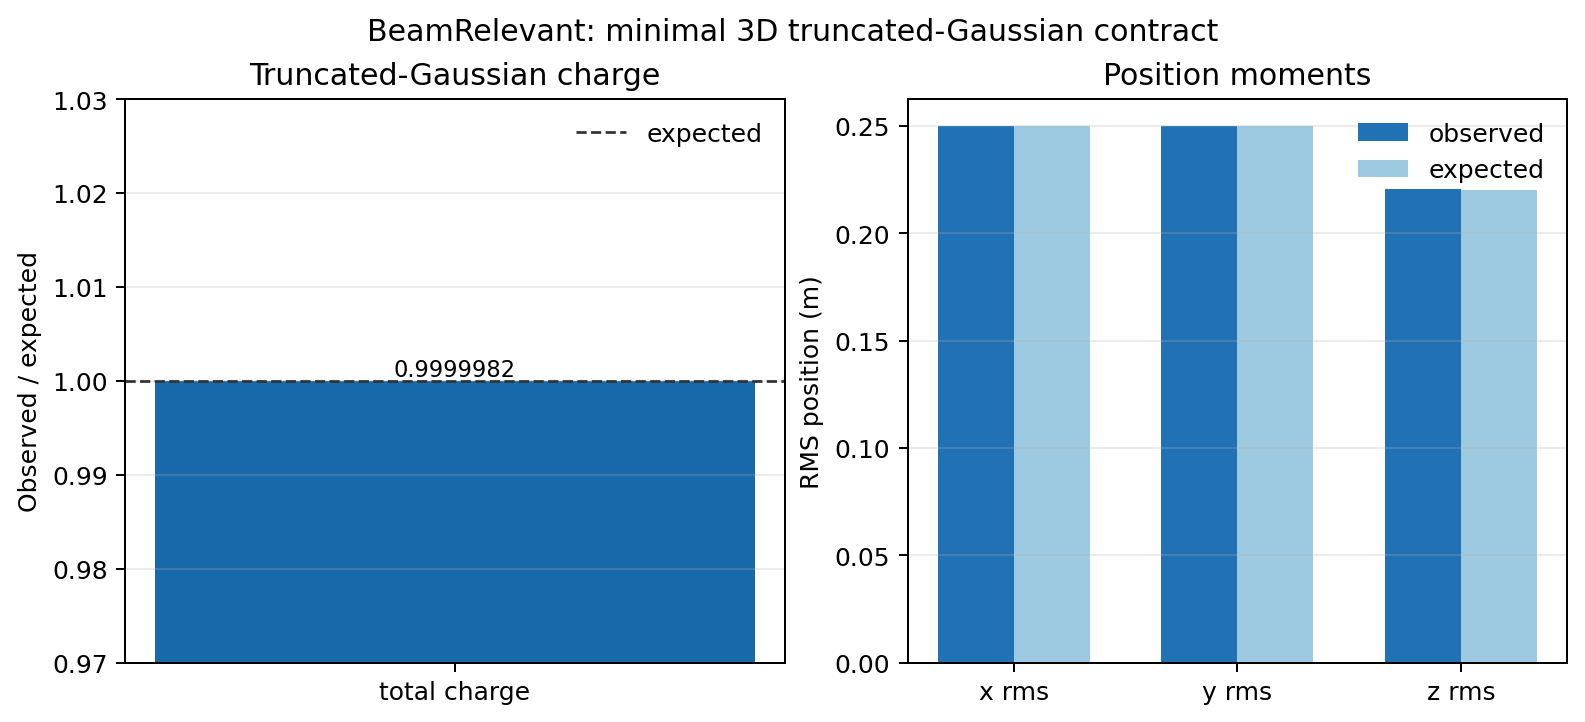
\includegraphics[width=0.8\linewidth]{../assets/figures/beam-relevant-contract.png}
\end{figure}

图 8-9 由 reader-side analysis 从对应的束流矩检查结果重新生成。

\subsection{Native external-file Gaussian beam：束斑理论包络检查}

\cpath{gaussian\_beam/CMakeLists.txt} 中的 native \cpath{test\_3d\_focusing\_gaussian\_beam\_from\_openpmd} 仍引用目录内不存在的 \cpath{analysis.py}，所以不能把它表述为已恢复的上游 CMake regression。可用的物理检查是：由 prepare 脚本和 native input 生成 plotfile 与 BP5 openPMD 输出，再用 reader-side analysis 独立读取 iteration 0 的 \cpath{x/y/z/w}，与理论束斑包络比较。

该输入产生 \code{1,999,966} 个宏粒子、总权重 \cpath{1.999966e10} 和 81 个有效 z slice；按 focal-distance 理论包络计算的最大相对误差为 \code{sigma_x = 3.0515e-2 < 0.051}、\code{sigma_y = 3.6214e-2 < 0.038}。官方 \cpath{analysis\_focusing\_beam.py} 也能处理同一输出。这个结果支持外部文件初始化后的束斑包络检查，但不表示缺失的上游 \cpath{analysis.py} 已恢复。

图 8-10 直接从同一 BP5 iteration 0 重建每个 z slice 的加权 \cpath{sigma\_x}、\cpath{sigma\_y}，并与 focal-distance 理论包络叠加。它展示外部文件初始化后的真实粒子输出与理论束斑的一致性，而不是替代缺失的上游 \cpath{analysis.py}。

\begin{figure}[htbp]
\centering
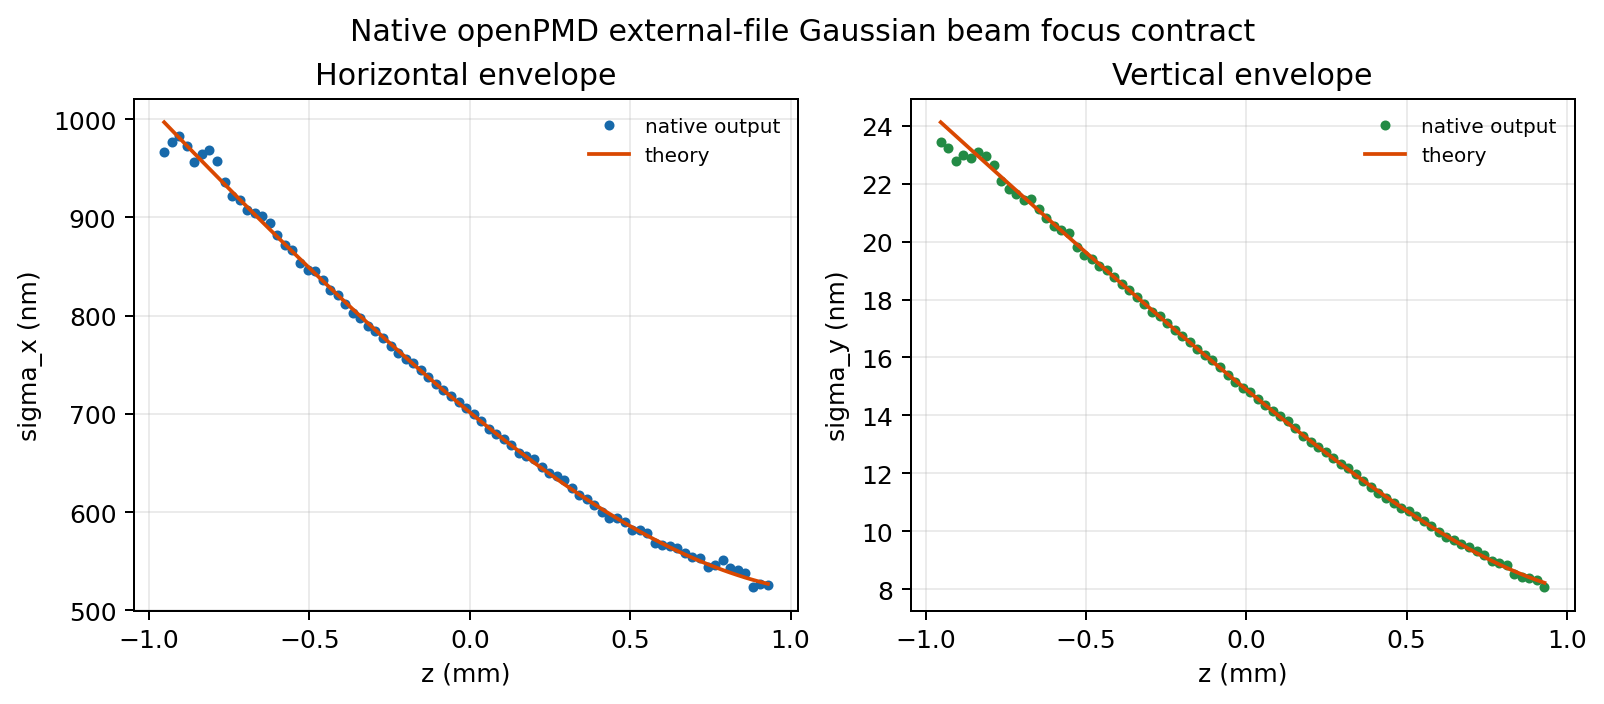
\includegraphics[width=0.8\linewidth]{../assets/figures/gaussian-beam-focus-contract.png}
\end{figure}

图 8-10 由 reader-side analysis 从对应的 Gaussian beam 输出重新生成。

完整官方 \cpath{Examples/Tests/initial\_distribution/} input 已由对应源码重建的 binary 复现。producer 和官方 \cpath{analysis.py} 均以 exit code \cpath{0} 结束，10 类分布的最大相对差为 \code{1.8931e-2 < 0.02}。仓库 checksum 默认 \cpath{rtol=1e-9} 观察到最大相对差 \cpath{3.18e-3}，反映随机采样而非初始化失败；在显式记录的 \cpath{rtol=5e-3} sampling tolerance 下通过。因此该案例的结论是“官方分布 analysis 通过、随机 checksum 有条件通过”，但不宣称确定性 \cpath{1e-9} checksum 相等。

\subsection{第 8 章验证矩阵：观察量、结论与边界}

详细输入、命令、环境和原始报告属于复现实验材料；正文只保留读者解释结果所需的观察量、结论与限制。

% <-- table block (source: 08-diagnostics-cases L1638)
\begin{tabularx}{\textwidth}{LLL}
\toprule
案例/诊断 & 观察量与可支持结论 & 仍需保留的边界 \\
\midrule
\endfirsthead
\toprule
案例/诊断 & 观察量与可支持结论 & 仍需保留的边界 \\
\midrule
\endhead
Langmuir & 场误差 \cpath{1.70e-3}、最终守恒 \cpath{8.35e-12}、频率误差 \cpath{3.595e-4}；解析波与守恒链均通过 & 不替代多模式或完整色散研究 \\
Uniform plasma restart & 同一 3D、2-rank CTest 布局中，遍历 level-0 \cpath{field\_list}，要求每个基线/restart 末态字段误差 \code{< 1e-12} & 不证明热平衡或跨布局物理等价 \\
Uniform plasma 跨布局 & 需要独立定义全局统计量、随机采样策略与容差 & 不能从 restart field-by-field PASS 推出 1-rank、2-rank 或其他分块的等价性 \\
Thermal plasma & \cpath{EF+EP} 共同漂移 \cpath{<0.003} & 仅覆盖指定 family 和时间窗 \\
FieldProbe & coarse \codeesc{3.6703\%} 失败；matched-time refined \codeesc{0.3533\%} 通过 & refined 结果不能反写为 coarse 输入通过 \\
Reduced observables & 60 项与 full-state reference 对照；非 field-energy \cpath{<1e-12} & field-energy 使用独立的 \cpath{<0.3} 容差 \\
LoadBalanceCosts & \code{eta_after > eta_before} & 验证效率改善，不验证场精度 \\
ColliderRelevant / DifferentialLuminosity & 束流统计与 1D/2D 解析谱交叉验证 & 不替代 collider-QED 应用级复现 \\
ParticleHistogram2D / BeamRelevant & writer schema、有限非零数据、截断 Gaussian charge/rms & 不给出粒子数正式收敛阶 \\
Initial distribution / Gaussian beam & 分布 analysis 与束斑理论包络通过 & 随机 checksum 与缺失上游 analysis 保持边界 \\
RZ sphere / RZ multimode & 场、rho-volume charge 与 mode writeback 的有界检查 & 不替代完整 RZ 诊断矩阵 \\
\bottomrule
\end{tabularx}

这张表中的“通过”只表示对应列出的 gate 通过。例如 FieldProbe 的 coarse 输入仍然是失败证据，完整 initial-distribution 的随机 checksum 也不等价于确定性 \cpath{1e-9} 回归；这样读者可以从同一张表直接区分强 physics analysis、writer/schema contract、性能 gate 和采样统计边界。任何摘要都不替代下表所指向的输入、analysis 和原始诊断输出。

本章的证据等级应按诊断问题分开理解：Langmuir 提供解析频率、场误差和最终守恒；uniform plasma 提供 Full diagnostics workflow 与同一布局下 checkpoint/restart 的逐字段一致性，但短时总能量变化不等于热平衡守恒，restart PASS 也不等于跨布局等价；FieldProbe 的 \cpath{lambda/32} matched-time 对照通过解析 gate，而官方 \cpath{lambda/16} coarse case 仍是失败证据；\cpath{reduced\_diags} 将 compact observable 与 full-state reference 逐项对照，\cpath{LoadBalanceCosts} 则只验证效率改善；\cpath{ColliderRelevant}、\cpath{DifferentialLuminosity}、\cpath{ParticleHistogram2D} 和 \cpath{BeamRelevant} 分别验证其统计、谱或 writer 定义。RZ 多模 Langmuir 和 native Gaussian sibling 是有界案例证据，不能替代各自缺失的官方 analysis。每一项都必须沿验证矩阵中的 producer、consumer、observable 和限制阅读，不能用“已经运行”替代物理结论。

\section{从诊断入口到可解释证据}

面对一个新案例，先不要从“它写出了哪个文件”开始判断结果，而要依次回答三个问题：

\begin{enumerate}
\item \textbf{要测的物理量是什么，处在哪个时间层？}主循环决定诊断何时采样；Full、BTD 与 BoundaryScraping 的差别决定你得到的是全状态、回到实验室系的快照，还是粒子边界事件。
\item \textbf{这个量怎样从模拟状态变成输出？}\cpath{ComputeDiagFunctors} 负责字段派生量，粒子采样和 \cpath{flush} 决定归约或 writer 的时机，OpenPMD iteration 则给出可由分析器读取的时间序列坐标。
\item \textbf{输出能够支持什么结论？}解析 comparison 是 physics evidence，writer/schema 检查说明数据形状可消费，checksum 说明指定输出回归，performance gate 只说明效率指标。它们不能互相升级。
\end{enumerate}

因此，\cpath{MultiDiagnostics} 或 \cpath{WarpXOpenPMD} 的入口存在，只说明诊断链被接入，不能反向证明每个下游案例都已通过。阅读验证矩阵时，应先从观察量和预期物理行为选择 case，再追踪生成该量的 consumer；不要把“文件已生成”误写为“物理机制已验证”。

\subsection{三类 reduced diagnostics 的最小起点}

三类 reduced diagnostics 的最小输入可以这样起步：

\begin{itemize}
\item \cpath{FieldProbe}：官方 reduced-diags 测试中的 point/line/plane 骨架；
\item \cpath{ParticleHistogram2D}：laser-ion 测试中的 \cpath{z}--\cpath{uz} openPMD mesh；
\item \cpath{LoadBalanceCosts}：\code{LBC.type = LoadBalanceCosts} 与官方 efficiency analysis。
\end{itemize}

这些最小输入只回答“怎样产生该类输出”。它们不替代 \cpath{FieldProbe} 的解析 diffraction gate，不把 \cpath{ParticleHistogram2D} 的 writer/schema 变成物理收敛证明，也不把 \cpath{LoadBalanceCosts} 的效率比较与场精度混为同一类 physics gate。

\subsection{一张诊断记录卡}

对任何一个新案例，都可以先写完下面五项，再决定是否值得扩大输出或运行时间：

% <-- table block (source: 08-diagnostics-cases L1680)
\begin{tabularx}{\textwidth}{LLL}
\toprule
项目 & 必须写清的内容 & 常见误读 \\
\midrule
\endfirsthead
\toprule
项目 & 必须写清的内容 & 常见误读 \\
\midrule
\endhead
物理问题 & 例如波频率、能量漂移、边界粒子通量或束流 rms & 把“已有一个输出文件”当成问题本身 \\
producer 与时间层 & 哪条推进/同步路径生成状态，Full、BTD、reduced 或 scraping 在何时采样 & 把同一 step 编号当作同一瞬时状态 \\
consumer 与比较量 & 哪个 analysis 或独立重建读取什么量，误差/守恒量/谱量怎样定义 & 只报告 writer 成功而不定义 observable \\
reference 与阈值 & 解析解、benchmark、restart sibling、full-state reference 或明确的性能目标 & 用 checksum 替代物理 reference \\
结论边界 & 已覆盖的几何、solver、分辨率、粒子数和未覆盖的分支 & 将局部 PASS 外推为所有设置都正确 \\
\bottomrule
\end{tabularx}

这张卡的作用不是增加一层文档，而是防止“输入、输出、比较和结论”在阅读中脱节。只有五项能逐一对应时，某个 PASS 才能被解释为可复查的证据；任何一项缺失，都应将结果降级为工作流、writer 或源码接线线索。

\subsection{修改诊断后的验证阶梯：先核 producer，再解释输出}

修改诊断代码或输入后，最常见的误读是“文件写出来了，所以物理量正确”。诊断跨越调度、归约/采样、writer 和 reader-side comparison；改动任一层，都应选择实际消费该层状态的检查。

\textbf{第一层：先确认调度与时间层真的到达。}\cpath{WarpX::Evolve()} 仅在 \cpath{DoComputeAndPack(step)} 或 \cpath{DoDiags(step)} 为真时列入诊断，必要时先同步速度；reduced diagnostics 走 \cpath{ComputeDiags()}/\cpath{WriteToFile()}，其余由 \cpath{FilterComputePackFlush()} 分派。改 \cpath{intervals}、\cpath{diag\_type}、writer 或同步条件时，先核输出的 step、时间、对象与字段。它只证明 producer 到达正确时间层，不能证明归约公式或参考量正确。

\textbf{第二层：改 compact reduced observable 时，以 full state 作 reference。}2-rank \cpath{test\_3d\_reduced\_diags} 同时输出 Full plotfile 与能量、动量、最大值、粒子数和 \cpath{FieldReduction}；分析器从 Full 重算并比较各文本列。除 staggered/cell-centered 的 field energy 用 \code{< 0.3} 外，其余默认 \code{< 1e-12}。它适合检查归约定义、加权、MPI reduction 与列写出，支持同一时刻的 compact/full-state 一致，不能代替其他 writer、interval、几何或守恒律验证。

\textbf{第三层：改 bin、轴标签或 openPMD reduced mesh 时，用解析谱而非文件形状验收。}3D、2-rank \cpath{test\_3d\_diff\_lumi\_diag\_leptons} 比较 128-bin 文本谱与 \code{128 x 128} openPMD 谱，核对二维轴顺序，并与 Gaussian-beam 解析谱比较；leptons 的 1D/2D 误差阈值为 \cpath{0.02}/\cpath{0.04}。它检验 binning、metadata 与聚合，不能推出其他 species、range、AMR 或 collider-QED application 已复现。

\textbf{第四层：改 sampling geometry、gather 或时间积分时，让 observable 匹配采样定义。}\cpath{test\_2d\_field\_probe} 在 step 500 读取 line probe；\code{integrate = 1} 给出 fluence，不是瞬时强度，analysis 以单缝 $\mathrm{sinc}^2$ 包络要求平均误差 \codeesc{< 2.5\%}。它检查 probe 几何、\cpath{E/B} gather、积分与坐标选择；文件生成不等于通过，改变积分或位置必须另建 reference。

\textbf{第五层：有跨步状态时，restart 与 checksum 只检查各自的生命周期。}2-rank \cpath{test\_3d\_uniform\_plasma\_restart} 从 \cpath{chk000006} 续跑，对同布局 level-0 \cpath{field\_list} 逐字段 \code{< 1e-12} 比较；checksum 以 \code{--rtol 1e-12} 锁定指定输出。累积量还须有 checkpoint hook，如 \cpath{FieldPoyntingFlux} 的读写接口。它们不能替代 full-state、解析谱或采样物理量。

按改动对象选层：scheduling/writer、reduced quantity、二维谱/bin/metadata、probe/integration、checkpoint/累计量依次对应第一至第五层。未执行 consumer 只能是“不适用或尚未执行”，不能把缺少 comparison 写成通过；所有层都不能替代跨分辨率、跨 MPI 布局或新的物理 reference。

\section{练习与复现实验}

\begin{enumerate}
\item \textbf{证据分层题}：从验证矩阵中各选一个 physics gate、writer/schema 检查和 performance gate，说明它们的 producer、analysis 量和“不能支持的结论”。
\item \textbf{reader-side 复现题}：使用官方 \cpath{analysis.py} 或独立的 reader-side analysis 读取一个案例输出，按诊断记录卡列出输入字段、采样时间层、输出文件、比较量、阈值和不可外推范围。
\item \textbf{失败边界题}：解释为什么 FieldProbe coarse failure、uniform-plasma 的跨布局问题和 initial-distribution binary mismatch 都应保留在书中，而不能简单从验证矩阵中删除。
\end{enumerate}

\section{延伸验证路线}

\begin{itemize}
\item 沿 \cpath{ComputeDiagFunctors/}、\cpath{ParticleIO}、\cpath{WarpXOpenPMD} 和 \cpath{FlushFormats/} 分开追踪字段计算、粒子采样与 writer 生命周期，避免把文件格式当成物理诊断。
\item 以 \cpath{FieldProbe}、\cpath{ParticleHistogram2D} 和 \cpath{LoadBalanceCosts} 的最小输入为例，分别复现解析 gate、writer/schema contract 和 performance gate。
\item 用更长的 uniform-plasma 时间窗，并结合 \cpath{energy\_conserving\_thermal\_plasma} 的 analysis，区分短时统计漂移与可解释的总能量结论。
\item 改变 Langmuir 的模式数和拟合时间窗，检验频率测量对 sampling window 的敏感性，避免把单一窗口拟合误读为完整色散验证。
\end{itemize}

\section{本章结论}

诊断的价值不在于输出文件越多，而在于每一个输出都与明确的物理问题、时间层和判据相连。读者可以用下面四步设计或审读一个诊断：

\begin{enumerate}
\item \textbf{先写问题和比较对象。}例如是 Langmuir 的解析频率、PML 的残余场、束流的相空间矩，还是 checkpoint/restart 的可重复性；不同问题要求不同 reference，而不是同一个通用 checksum。
\item \textbf{再选状态与时间层。}确定需要全场、粒子、reduced observable、BTD 还是 boundary event，并明确采样发生在推进、同步或输出的哪一个阶段。
\item \textbf{为结论配对证据等级。}物理 gate、writer/schema、性能量和输出回归应分别报告；只有与理论或独立 reference 比较的量才能支持相应的物理断言。
\item \textbf{保留失败与不可外推范围。}FieldProbe coarse failure、随机初始化的有限采样误差、跨 rank 的 field 差异和缺失的上游 analysis 都是结果的一部分。删除它们会让验证矩阵看似更整齐，却会削弱读者判断可信度的能力。
\end{enumerate}

这条路线把第 4--7 章的算法、沉积、场更新与边界条件接到第 8 章的可观测量上：只有先知道一个量在何处产生、何时同步、由哪个 writer 或 analysis 消费，才能解释它究竟在验证哪一段 PIC 链。第 9 章将进一步说明如何为这些结论选择文献证据，并区分全文、摘要和源码案例各自能支持的范围。
